\documentclass[aspectratio=169, table,colorlinks, 10pt, xcolor = table]{beamer}
\usetheme{Madrid} 

%% COLOR
\usepackage{fontawesome5}
\usepackage{adjustbox}
\usepackage{array}
\usepackage{ifthen}
\usepackage{colortbl}
\usepackage{adjustbox}
\usepackage{tikz-network}

%\definecolor{unipdcol}{rgb}{0.59, 0.0, 0.09}
\definecolor{unipdcol}{HTML}{253c5c}

\definecolor{newred}{rgb}{0.8,0,0}
\definecolor{avocado}{HTML}{2B7A0B}
\definecolor{newblue}{HTML}{0270c0}

\definecolor{INFBlue}{RGB}{0, 92, 161}
\definecolor{UFGBlue}{RGB}{0, 114, 185}
\definecolor{PrimaryColor}{RGB}{33, 33, 33}

\definecolor{DarkGray}{RGB}{33,33,33}
\definecolor{LightGray}{RGB}{150,150,150}
\definecolor{LightGray2}{RGB}{200,200,200}
\definecolor{Ocean}{RGB}{129,194,234}
\definecolor{DarkOrange}{RGB}{255, 152, 0}
\definecolor{LightOrange}{RGB}{255, 193, 7}
\definecolor{DarkGreen}{RGB}{91, 141, 8}
\definecolor{LightGreen}{RGB}{122, 188, 12}
\definecolor{LightPurple}{RGB}{191, 83, 219}
\definecolor{DarkPurple}{RGB}{142, 36, 170}
\definecolor{VeryLightGray}{RGB}{249, 249, 249}
\definecolor{mybluehl}{HTML}{cbd3ff}
\definecolor{newpink}{HTML}{ff5b77}


\DeclareMathOperator*{\argmin}{arg\,min}
\setbeamercolor{alerted text}{fg=DarkOrange}
\setbeamercolor{example text}{fg=DarkGreen}
\usepackage[normalem]{ulem}

\newcommand{\nologo}{\setbeamertemplate{logo}{}} % command to set the logo to nothing


%% THEME
\setbeamertemplate{navigation symbols}{}
\setbeamertemplate{headline}{}
\setbeamercolor{footer}{fg=white, bg=unipdcol}
\setbeamercolor{frametitle}{fg=white, bg =unipdcol}

\usecolortheme[named=unipdcol]{structure}
\makeatletter
\setbeamertemplate{footline}
{
  \leavevmode%
  \hbox{%
  \begin{beamercolorbox}[left, sep=0.1cm, wd=\textwidth]{footer}%
  	\ifbeamer@inappendix%
  	\hspace*{0.2cm}\usebeamerfont{author in head/foot}\scriptsize\insertshorttitle$\quad\mid\quad$\insertshortauthor
  \else%
    \hspace*{0.2cm}\usebeamerfont{author in head/foot}\scriptsize
    \ifx\insertsectionhead\@empty\insertshorttitle$\quad\mid\quad$\else\insertsectionhead$\quad\mid\quad$\fi \insertshortauthor\hspace{0pt plus 1 filll} \insertframenumber{} \hspace*{0.2cm} 
  \fi%
  \end{beamercolorbox}}%
  \vskip0pt%
}
\makeatother
\setbeamertemplate{blocks}[rounded][shadow=false]
\addtobeamertemplate{footline}{\hypersetup{allcolors=.}}{}
\addtobeamertemplate{frametitle}{\hypersetup{allcolors=.}}{}
\addtobeamertemplate{title page}{\hypersetup{allcolors=.}}{}

\newenvironment{variableblock}[3]{%
  \setbeamercolor{block body}{#2}
  \setbeamercolor{block title}{#3}
  \begin{block}{#1}}{\end{block}}
  
%\newcommand{\confname}{Conf name}
\makeatletter
\newcommand{\unilogo}{\@dblarg\beamer@unilogo}\long\def\beamer@unilogo[#1]#2{%
  \def\insertunilogo{#2}%
  \def\beamer@unilogo{#1}%
  \def\insertunilogo{#1}
  }
\makeatother

\setbeamertemplate{title page}{%
	\hypersetup{allcolors=.}
    \begin{tikzpicture}[remember picture,overlay]
    \draw[fill=unipdcol] (current page.south west) rectangle
  (current page.north east);
    \node[anchor=north, opacity = 0.3] at ([yshift=0.1\paperwidth, xshift=-0.25\paperwidth]current page.north east) {\includegraphics[width=0.8\paperwidth]{img/unipd3_black.png}};
    \node[inner xsep=15pt, inner ysep=40pt, text width=\paperwidth, align = left, anchor=north west, text=white, yshift = -0.5cm, execute at begin node=\setlength{\baselineskip}{6ex}] at (current page.north west) (title){\usebeamerfont{title}\Huge\bfseries\inserttitle};
    \node[inner xsep=15pt, inner ysep=20pt, text width=\paperwidth, align = left, text = white, anchor = north west, yshift = -4cm, execute at begin node=\setlength{\baselineskip}{2ex}] at (current page.north west) (auth){\usebeamerfont{author}\bfseries\insertauthor};
    \node[inner xsep=15pt, inner ysep=20pt, text width=\paperwidth, align = left, text = white, anchor = north west, yshift = -5.25cm] at (current page.north west) (ist){\usebeamerfont{author}\insertinstitute};
    \node[inner xsep=15pt, inner ysep=10pt, text width=\paperwidth, align = left, text = black, anchor = south west, fill = white] at (current page.south west) (conf){\insertdate};  
    \node[inner xsep=10pt, yshift = 0cm, text width=\paperwidth, align = right, text = black, anchor = south east] at (current page.south east) (uni){\includegraphics[width = 0.125\linewidth]{img/TAFSlogo2.png}};   
    \end{tikzpicture}
}

\makeatletter
\setbeamertemplate{frametitle}
{
  \hypersetup{allcolors=.}
  \ifbeamercolorempty[bg]{frametitle}{}{\nointerlineskip}%
  \@tempdima=\textwidth%
  \advance\@tempdima by\beamer@leftmargin%
  \advance\@tempdima by\beamer@rightmargin%
  \begin{beamercolorbox}[sep=0.3cm,left,wd=\the\@tempdima]{frametitle}
    \vbox{}\vskip-1ex%
    \if@tempswa\else\csname beamer@fteleft\endcsname\fi%
    {\strut\bfseries\insertframetitle\strut\par%
    {%
      \ifx\insertframesubtitle\@empty%
      \else%
      {\usebeamerfont{framesubtitle}\usebeamercolor[fg]{framesubtitle}\normalfont\insertframesubtitle\strut\par}%
      \fi
    }}%
    \vskip-1ex%
    %\rule{\dimexpr\paperwidth-0.6cm\relax}{0.8pt}}
    %\vskip-0.75ex%
    \if@tempswa\else\vskip-.3cm\fi% set inside beamercolorbox... evil here...
  \end{beamercolorbox}%
    %
}

\setbeamertemplate{block alerted begin}{
	\vspace{\fill}
	\begin{adjustbox}{max width=\textwidth, trim=0 2ex 0 0,clip}
		\begin{tabular}{!{\color{DarkOrange}{\vrule width 4pt}}>{\columncolor{DarkOrange!10}}m{\linewidth}}
			\begin{beamercolorbox}{alerted text} \usebeamerfont*{block title} \vbox{}\vskip 0.2ex \bfseries \insertblocktitle \end{beamercolorbox}\usebeamerfont*{block text}
		}
		\setbeamertemplate{block alerted end}{\end{tabular}\end{adjustbox}}
		
\setbeamertemplate{block example begin}{
	\vspace{\fill}
	\begin{adjustbox}{width=\linewidth, trim=0 2ex 0 0,clip}
		\begin{tabular}{!{\color{DarkGreen}{\vrule width 4pt}}>{\columncolor{DarkGreen!10}}m{\textwidth}}
			\begin{beamercolorbox}{example text} \usebeamerfont*{block title} \vbox{}\vskip 0.2ex \bfseries \insertblocktitle \end{beamercolorbox}\usebeamerfont*{block text} 
		}
\setbeamertemplate{block example end}{\end{tabular}\end{adjustbox}}
\makeatother


\hypersetup{allcolors=.,
			citecolor = .}

%% TABLE
\usepackage{booktabs}
\newcolumntype{M}[1]{>{\centering\arraybackslash}m{#1}}
\newcolumntype{L}[1]{>{\raggedright\arraybackslash}m{#1}}
\newcolumntype{R}[1]{>{\raggedleft\arraybackslash}m{#1}}
\newcolumntype{P}[1]{>{\centering\arraybackslash}p{#1}}
\usepackage{multirow}
\usepackage{colortbl}

\renewcommand<>\rowcolor[1]{\only#2{\\[-\normalbaselineskip]\beameroriginal\rowcolor{#1}}}

\renewcommand<>\cellcolor[1]{\only#2{\beameroriginal\cellcolor{#1}}}
%% BIB
\usepackage[authoryear,round]{natbib}

%% ITEMIZE
\setbeamercolor{itemize item}{fg=black}
\setbeamertemplate{itemize item}[square]
\setbeamertemplate{itemize subitem}[circle]
\setbeamertemplate{itemize subsubitem}[triangle]


\setbeamercolor{enumerate item}{fg=black}
\setbeamertemplate{enumerate item}[circle]
\setbeamertemplate{sections/subsections in toc}[square]
\setbeamertemplate{section in toc}[sections numbered]

\usepackage{enumitem}
\setitemize{label=\usebeamerfont*{itemize item}%
	\usebeamercolor[fg]{itemize item}
	\usebeamertemplate{itemize item}}
\setlist[enumerate,1]{%
	label=\protect\usebeamerfont{enumerate item}%
	\protect\usebeamercolor[fg]{enumerate item}%
	\insertenumlabel.%
}

%% TIKZ
\usepackage{tikz}
\usetikzlibrary{arrows, shapes, positioning, shadows, backgrounds, trees, shapes.misc, arrows.meta, calc, fit, patterns, patterns.meta, hobby}

\usetikzlibrary{matrix, decorations.pathreplacing, decorations.pathmorphing, decorations.markings}


\tikzset{
  basic/.style  = {draw, text width=2cm, drop shadow, font=\sffamily, rectangle},
  root/.style   = {basic, rounded corners=2pt, thin, align=center,
                   fill=green!30},
  level 2/.style = {basic, rounded corners=6pt, thin,align=center, fill=green!60,
                   text width=4em},
  level 3/.style = {basic, thin, align=left, fill=pink!60, text width=1.5em}
}
\newcommand{\relation}[3]
{
	\draw (#3.south) -- +(0,-#1) -| ($ (#2.north) $)
}
\newcommand{\relationBOLD}[3]
{
	\draw[line width = 0.1cm] (#3.south) -- +(0,-#1) -| ($ (#2.north) $)
}
\newcommand{\relationP}[3]
{
	\draw (#3.south) -- +(0,-#1) -| (#2.north)
}
\newcommand{\relationW}[2]
{
	\draw (#2.west) -| ($ (#1.north) $)
}
\newcommand{\relationE}[2]
{
	\draw (#2.east) -| ($ (#1.north) $)
}
\newcommand{\relationD}[3]
{
	\draw (#3.east) -- +(#1,0) |- (#2.west)
}
\pgfdeclareimage[height=0.4cm]{ngreen2}{img/boot/ngreen.pdf}
\pgfdeclareimage[height=0.4cm]{nblue2}{img/boot/nblue.pdf}
\pgfdeclareimage[height=0.4cm]{nred2}{img/boot/nred.pdf}
\pgfdeclareimage[height=0.4cm]{nblack2}{img/boot/nblack.pdf}

% Required packages
\usepackage{pgfplots}
\pgfplotsset{compat = newest}
\usepackage{soul}

%% Math symbol
\usepackage{bm}
\newcommand{\avet}{\bm{a}}
\newcommand{\bvet}{\bm{b}}
\newcommand{\cvet}{\bm{c}}
\newcommand{\dvet}{\bm{d}}
\newcommand{\evet}{\bm{e}}
\newcommand{\pvet}{\bm{p}}
\newcommand{\fvet}{\bm{f}}
\newcommand{\tvet}{\bm{t}}
\newcommand{\uvet}{\bm{u}}
\newcommand{\vvet}{\bm{v}}
\newcommand{\wvet}{\bm{w}}
\newcommand{\xvet}{\bm{x}}
\newcommand{\yvet}{\bm{y}}
\newcommand{\zvet}{\bm{z}}
\newcommand{\Avet}{\bm{A}}
\newcommand{\Bvet}{\bm{B}}
\newcommand{\Cvet}{\bm{C}}
\newcommand{\Dvet}{\bm{D}}
\newcommand{\Evet}{\bm{E}}
\newcommand{\Fvet}{\bm{F}}
\newcommand{\Gvet}{\bm{G}}
\newcommand{\Hvet}{\bm{H}}
\newcommand{\Ivet}{\bm{I}}
\newcommand{\Jvet}{\bm{J}}
\newcommand{\Kvet}{\bm{K}}
\newcommand{\Lvet}{\bm{L}}
\newcommand{\Mvet}{\bm{M}}
\newcommand{\Nvet}{\bm{N}}
\newcommand{\Pvet}{\bm{P}}
\newcommand{\Qvet}{\bm{Q}}
\newcommand{\Rvet}{\bm{R}}
\newcommand{\Svet}{\bm{S}}
\newcommand{\Tvet}{\bm{T}}
\newcommand{\Uvet}{\bm{U}}
\newcommand{\Wvet}{\bm{W}}
\newcommand{\Xvet}{\bm{X}}
\newcommand{\Yvet}{\bm{Y}}
\newcommand{\Zvet}{\bm{Z}}
\newcommand{\Zerovet}{\bm{0}}
\newcommand{\Omegavet}{\bm{\Omega}}
\newcommand{\betavet}{\bm{\beta}}
\newcommand{\epsvet}{\bm{\varepsilon}}
\newcommand{\etavet}{\bm{\eta}}
\newcommand{\alphavet}{\bm{\alpha}}
\newcommand{\lambdavet}{\bm{\lambda}}
\newcommand{\Unovet}{\bm{1}}
\newcommand{\Sigmavet}{\bm{\Sigma}}
\newcommand{\phivet}{\bm{\phi}}
\usepackage{mathpazo}

\newcommand\norm[1]{\lVert#1\rVert}

\usepackage{appendixnumberbeamer}

\title[Cross-temporal probabilistic forecast reconciliation]{\fontsize{27}{30}\selectfont Cross-temporal probabilistic \newline forecast reconciliation}
\author[Daniele Girolimetto]{{\Large Daniele Girolimetto}\\[0.1cm] 
{\normalfont\normalsize Department of Statistical Sciences, University of Padova}\\
{\normalfont\normalsize\href{https://danigiro.github.io/}{~\,\faGlobe~\texttt{danigiro.github.io}} \\
\href{https://github.com/danigiro}{~\,\faGithub~\texttt{danigiro}} \\
\href{mailto:daniele.girolimetto@unipd.it}{~\,\faAt~\texttt{daniele.girolimetto@unipd.it}}}}
\date{\textit{April 16$^{th}$, 2024} \\[0.15cm] \textbf{\large Time series Analysis and Forecasting Society}}
\unilogo{\includegraphics[width = 3.75cm]{img/unipd800.png}}

\logo{\vspace*{-0.2cm}\includegraphics[width = 1cm]{img/TAFSlogo2.png}}


\usepackage{makecell}

\begin{document}
\begin{frame}[plain, label = titlep]
   \maketitle
\end{frame}

\begin{frame}{Forthcoming paper}

\begin{minipage}{0.35\linewidth}\centering
	\includegraphics[width = 0.9\linewidth]{img/ijf.jpg}
\end{minipage}\begin{minipage}{0.65\linewidth}
\begin{itemize}
	\item[{\faIcon*[regular]{file}}] Girolimetto, D., Athanasopoulos, G., Di Fonzo, T., \& Hyndman, R. J. (2023). Cross-temporal probabilistic forecast reconciliation: Methodological and practical issues. International Journal of Forecasting. \href{https://doi.org/10.1016/j.ijforecast.2023.10.003}{\color{newblue}\texttt{DOI:10.1016/j.ijforecast.2023.10.003}}
\end{itemize}
\vskip0.5cm
\centering
    \hspace{0.5cm}\begin{tikzpicture}
    \node[align = center, anchor=center, label = {[font=\small, text width=25mm, align = center]below:{\textbf{Prof. George Athanasopoulos}}}] (george){\includegraphics[height = 0.3\linewidth]{img/george}};
    \node[align = center, anchor=center, right= 0.75cm of george, label = {[font=\small, text width=25mm, align = center]below:{\textbf{Prof. Tommaso \\ Di Fonzo}}}] (tommy){\includegraphics[height = 0.3\linewidth]{img/tommy}};
    \node[align = center, anchor=center, right= 0.75cm of tommy, label = {[font=\small, text width=25mm, align = center]below:{\textbf{Prof. Rob J \\ Hyndman}}}] (rob){\includegraphics[height = 0.3\linewidth]{img/rob}};
    \end{tikzpicture}
\end{minipage}
\end{frame}

\begin{frame}{Roadmap}
	\tableofcontents
    \begin{tikzpicture}[remember picture,overlay]
    \node[inner xsep=25pt, inner ysep=25pt, text width=\paperwidth, align = right, text = black, anchor = south east] at (current page.south east) (uni){\includegraphics[width = 0.2\linewidth]{img/logoFoReco.pdf}};   
    \end{tikzpicture}
\end{frame}

\section{Introduction}

\begin{frame}{Introduction}

\begin{itemize}[itemsep = 0.25cm]
	\item Forecast reconciliation is a post-forecasting process aimed to improve the quality of the base forecasts (however obtained) of a {\color{newblue}linearly constrained} multiple time series by exploiting cross-sectional (e.g., spatial) and/or temporal constraints of the {\color{newblue}target} forecasts
	\begin{center}
	\textbf{cross-sectional} framework $+$ \textbf{temporal} framework $\Rightarrow$ \textbf{cross-temporal} framework
	\end{center}
		\item Hot topic on forecasting methodology and practice:\\[0.1cm]
		\hspace{1.5cm}\faArrowRight\quad several contributions starting from {\color{newblue}\cite{hyndman2011}}\\[0.1cm]
	 %\item Looking for {\color{newblue}statistically well-grounded}, {\color{newblue}feasible} (practical implementation), {\color{newblue}effective} (quality of the results) approaches
	 \item Many forecasting applications: sales, production, tourism, energy demand, healthcare, real estate, supply chain, macroeconomics, $\dots$
	%\item {\color{newblue}Point} and {\color{newblue}probabilistic} forecast reconciliation
	\end{itemize}
	\vskip0.25cm
\begin{exampleblock}{\normalsize Hands on the Monthly Australian Tourism Demand dataset}
\begin{itemize}[nosep]
	\item Monthly data on visitor night from $1998 - 2017$
	\item From National Visitor Survey, annual interviews of 120,000 Australians aged 15+
	\item Source: \href{https://robjhyndman.com/data/TourismData_v3.csv}{\color{newblue}\texttt{robjhyndman.com/data/TourismData\_v3.csv}}
\end{itemize}
\end{exampleblock}
\end{frame}

\section{Cross-sectional, temporal and cross-temporal framework}

\begin{frame}[label = {cap:cs}]{Cross-sectional framework}{\cite{hyndman2011, panagiotelis2021, giro2022}}
\begin{minipage}{0.35\linewidth}\centering
	\includegraphics[width = \linewidth]{img/ausreg2.pdf}\\[0.5cm]
	\textit{States and territories of Australia: \\7 states and 76 regions}
\end{minipage}\hfill\begin{minipage}{0.625\linewidth}
\textbf{Notation}
\begin{itemize}
	\item $\yvet_t = $ vector of all ($n$) series at time $t$
	\item $\bvet_t = $ vector of the most disaggregated ($n_b$) series at time $t$
	\item $\avet_t = $ vector of the aggregated ($n_a = n - n_b$) series at time $t$
	\item Two equivalent representations
	\begin{enumerate}[itemsep = 0.25cm, topsep = 0.25cm]
		\item \textbf{Structural representation}: $\yvet_t = \Svet \bvet_t$\\[0.15cm] $\Svet = $ ($n \times n_b$) “structural matrix”
		\item \textbf{Zero-constrained representation}: $\Uvet'\mathbf{y}_t = \mathbf{0}_{(n_a \times n)}$\\[0.15cm] $\Uvet'$ = ($n_a \times n$) “zero-constrained matrix” containing the linear constraints ($n_a = n - n_b$)
	\end{enumerate}
\end{itemize}
\end{minipage}
\end{frame}

\begin{frame}[fragile]{Hierarchical and grouped time series}
\centering
\textit{Genuine hierarchical time series}\\
\begin{minipage}{0.49\linewidth}
\centering
	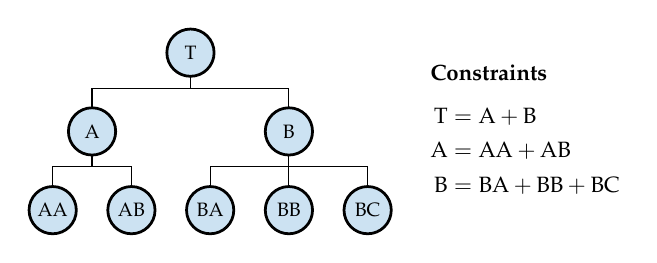
\begin{tikzpicture}
		\Vertex[y = 2, x = 1.75, label=T, color = newblue, opacity = 0.2]{T}
		\Vertex[x=0.5,y=1, label = A, color = newblue, opacity = 0.2]{A}
		\Vertex[x=3, y = 1, label = B, color = newblue, opacity = 0.2]{B}
		\Vertex[x=0, y = 0, label = AA, color = newblue, opacity = 0.2]{AA}
		\Vertex[x=1, y = 0, label = AB, color = newblue, opacity = 0.2]{AB}
		\Vertex[x=2, y = 0, label = BA, color = newblue, opacity = 0.2]{BA}
		\Vertex[x=3, y = 0, label = BB, color = newblue, opacity = 0.2]{BB}
		\Vertex[x=4, y = 0, label = BC, color = newblue, opacity = 0.2]{BC}
	\relation{0.15}{AA}{A};
	\relation{0.15}{AB}{A};
	\relation{0.15}{BC}{B};
	\relation{0.15}{BA}{B};
	\relation{0.15}{BB}{B};
	\relation{0.15}{A}{T};
	\relation{0.15}{B}{T};
	\node[font = \footnotesize] at (6, 1) (cons){$\begin{aligned}
		\multicolumn{2}{l}{\textbf{Constraints}}\\[0.1cm]
		\text{T} &= \text{A} + \text{B}\\
		\text{A} &= \text{AA} + \text{AB}\\
		\text{B} &= \text{BA} + \text{BB} + \text{BC}
	\end{aligned}
	$};
	\end{tikzpicture}
\end{minipage}\hspace{0.5cm}
\begin{minipage}{0.4\linewidth}
	\begin{exampleblock}{}
A cross-sectional hierarchical/grouped time series is a collection of $n$ variables for which - at each time - \textbf{aggregation relationships} hold
\end{exampleblock}
\end{minipage}
\begin{center}
\textit{Grouped time series: two or more genuine hierarchies sharing the same top and bottom variables}\\
	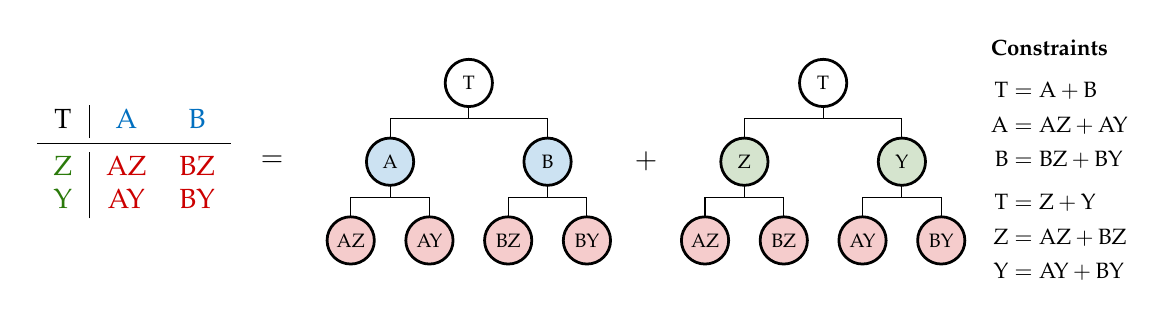
\begin{tikzpicture}
	\node[font = \normalsize] at (-2.75, 1) (ug){\begin{tabular}{c|cc}
	T & \textcolor{newblue}{A} & \textcolor{newblue}{B} \\
	\midrule
	\textcolor{avocado}{Z} & \textcolor{newred}{AZ} & \textcolor{newred}{BZ} \\
	\textcolor{avocado}{Y} & \textcolor{newred}{AY} & \textcolor{newred}{BY}
\end{tabular}};
	\node[font = \normalsize] at (-1, 1) (ug){$=$};
	\Vertex[y = 2, x = 1.5, label=T, color = white, opacity = 0.2]{T}
	\Vertex[x=0.5,y=1, label = A, color = newblue, opacity = 0.2]{A}
	\Vertex[x=2.5, y = 1, label =B, color = newblue, opacity = 0.2]{B}
	\Vertex[x=0, y = 0, label = AZ, color = newred, opacity = 0.2]{AZ}
	\Vertex[x=1, y = 0, label = AY, color = newred, opacity = 0.2]{AY}
	\Vertex[x=2, y = 0, label = BZ, color = newred, opacity = 0.2]{BZ}
	\Vertex[x=3, y = 0, label = BY, color = newred, opacity = 0.2]{BY}
	\relation{0.15}{AZ}{A};
	\relation{0.15}{AY}{A};
	\relation{0.15}{BZ}{B};
	\relation{0.15}{BY}{B};
	\relation{0.15}{A}{T};
	\relation{0.15}{B}{T};
	\node[font = \normalsize] at (3.75, 1) (plus){$+$};
	\Vertex[x=4.5, y = 0, label = AZ, color = newred, opacity = 0.2]{AZ1}
	\Vertex[x=5.5, y = 0, label = BZ, color = newred, opacity = 0.2]{BZ1}
	\Vertex[x=6.5, y = 0, label = AY, color = newred, opacity = 0.2]{AY1}
	\Vertex[x=7.5, y = 0, label = BY, color = newred, opacity = 0.2]{BY1}
	\Vertex[y = 2, x = 6, label=T, color = white, opacity = 0.2]{T1}
	\Vertex[x=5, y=1, label = Z, color = avocado, opacity = 0.2]{Z}
	\Vertex[x=7, y = 1, label =Y, color = avocado, opacity = 0.2]{Y}
	\relation{0.15}{AZ1}{Z};
	\relation{0.15}{AY1}{Y};
	\relation{0.15}{BZ1}{Z};
	\relation{0.15}{BY1}{Y};
	\relation{0.15}{Z}{T1};
	\relation{0.15}{Y}{T1};
	\node[font = \footnotesize] at (9, 1) (cons){$\begin{aligned}
		\multicolumn{2}{l}{\textbf{Constraints}}\\[0.1cm]
		\text{T} &= \text{A} + \text{B}\\
		\text{A} &= \text{AZ} + \text{AY}\\
		\text{B} &= \text{BZ} + \text{BY}\\[0.1cm]
		\text{T} &= \text{Z} + \text{Y}\\
		\text{Z} &= \text{AZ} + \text{BZ}\\
		\text{Y} &= \text{AY} + \text{BY}\\
	\end{aligned}
	$};
\end{tikzpicture}
\end{center}
\end{frame}

\begin{frame}[fragile]{Grouped time series}{Two or more genuine hierarchies sharing the same top and bottom variables}

For hierarchical/grouped time series where an aggregation matrix is always available ($\Avet$), the two representations are easily interchangeable:
$$
\underbrace{\Cvet:\;\avet_t = \Cvet\bvet_t}_{\substack{\scriptsize \text{Linear combination} \\[0.1cm] \text{(or aggregation) matrix}}} \qquad \Rightarrow \qquad 
\Svet = \begin{bmatrix}
\Cvet \\
\Ivet_{n_b}
\end{bmatrix} \qquad \text{and} \qquad \Uvet' = \begin{bmatrix}
\Ivet_{n_a} & -\Cvet
\end{bmatrix} 
$$

\vskip0.25cm

Structural and zero-constrained representations in \texttt{FoReco}:
\begin{center}
\begin{minipage}{0.475\linewidth}
\includegraphics[width = \linewidth]{img/code/Untitled2.png}
\end{minipage}
\quad\faArrowRight\qquad
\begin{minipage}{0.4\linewidth}\scriptsize
\begin{verbatim}
List of 6
 |-S : num [1:9, 1:4] 1 1 0 1 0 1 0 0 0 1 ...
 |-C : num [1:5, 1:4] 1 1 0 1 0 1 1 0 0 1 ...
 |-Ut: num [1:5, 1:9] 1 0 0 0 0 0 1 0 0 0 ...
 |-n : int 9
 |-na: int 5
 |-nb: int 4
\end{verbatim}
\end{minipage}	
\end{center}
\end{frame}

\begin{frame}[fragile]{General linearly constrained time series}{E.g.: two hierarchies that share only the most most aggregated level}
\begin{center}
\begin{minipage}{0.49\linewidth}\centering
\resizebox{0.9\linewidth}{!}{
	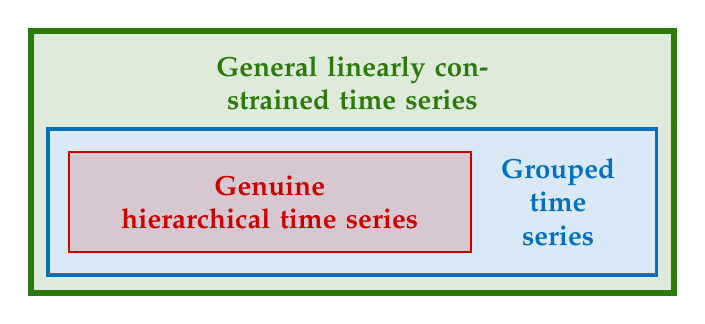
\begin{tikzpicture}
		\pgfdeclarelayer{background layer}
		\pgfdeclarelayer{backbackground layer}
		\pgfsetlayers{backbackground layer, background layer,main}
		\node[fill = newred, line width=0.25mm, fill opacity = 0.15, text opacity = 1, color = newred, draw, font = \bfseries, text width = 4.5cm, inner sep=3mm, align = center] (hts){Genuine \\hierarchical time series};
		\node[color = newblue, right = 0.1cm of hts, text width = 1.75cm, align = center, font = \bfseries] (lab_gts){Grouped time series};
		\begin{pgfonlayer}{background layer}
		\node[draw, line width=0.5mm, color = newblue, fill = newblue!15, inner sep=2.5mm,fit=(hts) (lab_gts)] (gts) {};	
		\end{pgfonlayer}
		\node[color = avocado, above = 0.1cm of gts, text width = 6.5cm, align = center, font = \bfseries] (labGLC){General linearly constrained time series};
		\begin{pgfonlayer}{backbackground layer}
		\node[draw, color = avocado, fill = avocado!15, inner sep=2mm, line width=0.75mm,fit=(hts) (lab_gts) (gts) (labGLC)] (GLC) {};	
		\end{pgfonlayer}
	\end{tikzpicture}}
\end{minipage}\begin{minipage}{0.49\linewidth}\centering
	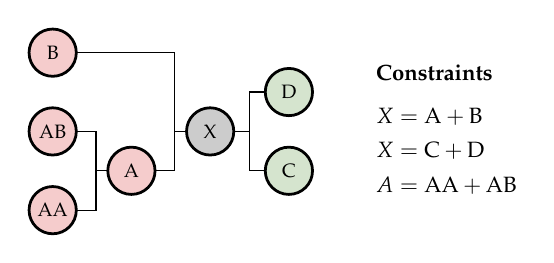
\begin{tikzpicture}	
		\Vertex[x=0,y=0, label = AA, color = newred, opacity = 0.2]{A1}
		\Vertex[x=0, y = 1, label = AB, color = newred, opacity = 0.2]{A2}
		\Vertex[x=0, y = 2, label = B, color = newred, opacity = 0.2]{B}
		\Vertex[x=3, y = 0.5, label = C, color = avocado, opacity = 0.2]{C}
		\Vertex[x=3, y = 1.5, label = D, color = avocado, opacity = 0.2]{D}
		\Vertex[x=1, y = 0.5, label = A, color = newred, opacity = 0.2]{A}
		\Vertex[x=2, y = 1, label = X, color = black!20]{X}
			
		\relationD{0.25}{A}{A1};
		\relationD{0.25}{A}{A2};
		\relationD{0.2}{C}{X};
		\relationD{0.2}{D}{X};
		\relationD{0.25}{X}{A};
		\relationD{1.25}{X}{B};
		\node[font = \footnotesize] at (5, 1) (cons){$\begin{aligned}
		\multicolumn{2}{l}{\textbf{Constraints}}\\[0.1cm]
		X &= \text{A} + \text{B}\\
		X &= \text{C} + \text{D}\\
		A &= \text{AA} + \text{AB}\\
	\end{aligned}
	$};
	\end{tikzpicture}
\end{minipage}
\end{center}
\begin{itemize}
\item Forecast reconciliation may be {\color{avocado}always} expressed according to a \textbf{zero-constrained} framework	
\end{itemize}
\begin{center}
\begin{minipage}{0.475\linewidth}
\includegraphics[width = \linewidth]{img/code/Untitled3.png}
\end{minipage}
\quad\faArrowRight\qquad
\begin{minipage}{0.4\linewidth}\scriptsize
\begin{verbatim}
List of 6
 |-Ut: num [1:3, 1:7] 1 0 0 0 1 0 0 0 1 -1 ...
 |-n : int 7
 |-na: int 3
 |-nb: int 4
\end{verbatim}
\end{minipage}	
\end{center}
\begin{itemize}
\item A \textbf{structural-like} representation may be derived:
\end{itemize}
\begin{center}
	\includegraphics[width = 0.475\linewidth]{img/code/Untitled4.png}
\end{center}
\end{frame}

\begin{frame}{Temporal framework}{\cite{athanasopoulos2017}}

\begin{minipage}{0.4\linewidth}
\centering
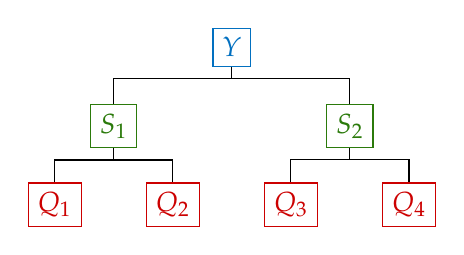
\begin{tikzpicture}[baseline=(current  bounding  box.center),
every node/.append style={shape=rectangle,
	draw=black},
minimum size=0.01cm]

\node[color=newred] at (0, 1) (Q1){$Q_1$};
\node[color=newred] at (1.5, 1) (Q2){$Q_2$};
\node[color=newred] at (3, 1) (Q3){$Q_3$};
\node[color=newred] at (4.5, 1) (Q4){$Q_4$};

\node[color=avocado] at (0.75, 2)  (S1){$S_1$};
\node[color=avocado] at (3.75, 2) (S2){$S_2$};

\node[color=newblue] at (2.25, 3) (A){$Y$};
\relation{0.15}{Q1}{S1};
\relation{0.15}{Q2}{S1};
\relation{0.15}{Q3}{S2};
\relation{0.15}{Q4}{S2};
\relation{0.15}{S1}{A};
\relation{0.15}{S2}{A};
\end{tikzpicture}
\\
\vskip0.2cm
{\footnotesize Quarterly hierarchy: \\[-0.1cm] {\color{newred}quarterly}, {\color{avocado}semi-annual} and {\color{newblue}annual} series}
\end{minipage}
\begin{minipage}{0.59\linewidth}
	\begin{exampleblock}{}
\textbf{Temporal hierarchy} \faArrowRight \; \textbf{non-overlapping aggregation} of the observations of a time series ($\yvet_i$) at regular intervals
$$
x_{i,\tau}^{[k]} = \displaystyle\sum_{t=(\tau-1)k+1}^{\tau k} y_{i,t} \qquad\text{for}\qquad \tau = 1,\dots \lfloor T/k \rfloor
$$\\[-0.25cm]
\textbf{NB:} \; For $k = 1$, $\tau = t = 1, \dots, T$ and $x_{i,\tau}^{[1]} = y_{i,t}$
\end{exampleblock}
\end{minipage}
\begin{itemize}[topsep=0.35cm, itemsep = 0.2cm]
	\item $k \in \mathcal{K} = \{k_p, \dots, k_1\}$ denote the $p$ factors of $m$ in descending order, where $k_1 = 1$ and $k_p = m$
	\item $k^\ast = \sum_{k \in \mathcal{K} \backslash \{k_1\}} k$ is the number of upper time series of the temporal hierarchy
	\item Unlike cross-sectional hierarchies (\textbf{$n$ variables at the same time index} are considered), in temporal hierarchies we have \textbf{one variable observed at different frequencies}
\end{itemize}
\end{frame}

\begin{frame}[fragile]{Temporal matrices: quarterly data}
\vspace{-0.5cm}
$$
\xvet_{i,\tau} = \begin{bmatrix}
	{\color{newblue}x_{i,\tau}^{[m]}}\\[0.2cm]
	{\color{avocado}\xvet_{i,\tau}^{[k_{p-1}]}}\\
	\vdots\\
	{\color{avocado}\xvet_{i,\tau}^{[k_{2}]}}\\[0.2cm]
	{\color{newred}\xvet_{i,\tau}^{[1]} = \yvet_{i,\tau}}\\
\end{bmatrix} = \begin{bmatrix}
	{\color{newblue}x_{i,\tau}^{[4]}}\\
	{\color{avocado}x_{i,2(\tau-1)+1}^{[2]}}\\
	{\color{avocado}x_{i,2(\tau-1)+2}^{[2]}}\\[-0.15cm]
	{\color{newred}y_{i,4(\tau-1)+1}^{\phantom{[1]}}}\\[-0.15cm]
	{\color{newred}y_{i,4(\tau-1)+2}^{\phantom{[1]}}}\\[-0.15cm]
	{\color{newred}y_{i,4(\tau-1)+3}^{\phantom{[1]}}}\\[-0.15cm]
	{\color{newred}y_{i,4(\tau-1)+4}^{\phantom{[1]}}}\\
\end{bmatrix}
\qquad
\begin{aligned}
	\Kvet &= \begin{bmatrix}
	\Unovet_m'\\
	\Ivet_{\frac{m}{k_{p-1}}}\otimes\Unovet_{k_{p-1}}'\\
	\vdots\\
	\Ivet_{\frac{m}{k_{2}}}\otimes\Unovet_{k_{2}}'
\end{bmatrix}  = 
\begin{bmatrix}
	{\color{newblue}1} & {\color{newblue}1} & {\color{newblue}1} & {\color{newblue}1} \\
	{\color{avocado}1} & {\color{avocado}1} & {\color{avocado}0} & {\color{avocado}0} \\
	{\color{avocado}0} & {\color{avocado}0} & {\color{avocado}1} & {\color{avocado}1}  \\
\end{bmatrix}\\[0.5cm]
\tau &= 1, \dots,  \lfloor T/m \rfloor
\end{aligned}
$$
\begin{minipage}{0.6\linewidth}
\begin{itemize}[leftmargin = 0.5cm]
\item $\tau$ is the time index for the most aggregated series, $i$ is the cross-sectional index, $M_k = m/k$ is the seasonal period of aggregated series
\item {\color{avocado}Structural}, $\xvet_{i,\tau} = \Rvet\xvet^{[1]}_{i,\tau}$, and {\color{avocado}zero-constrained}, $\Zvet'\xvet_{i,\tau} = \Zerovet$, representations still hold, and may be alternatively used for reconciliation
\end{itemize}
\end{minipage}\begin{minipage}{0.4\linewidth}
\centering
	\includegraphics[width = 0.9\linewidth]{img/code/Untitled5.png}\\
	\begin{minipage}{0.8\linewidth}\tiny
	\begin{verbatim}
List of 8
 |-K   : num [1:3, 1:4] 1 1 0 1 1 0 1 0 1 1 ...
 |-Zt  : num [1:3, 1:7] 1 0 0 0 1 0 0 0 1 -1 ...
 |-R   : num [1:7, 1:4] 1 1 0 1 0 0 0 1 1 0 ...
 |-kset: int [1:3] 4 2 1
 |-m   : num 4
 |-p   : int 3
 |-ks  : num 3
 |-kt  : num 7
\end{verbatim}
\end{minipage}
\end{minipage}
\end{frame}

\begin{frame}[label = {cap:figCT}]{\hyperlink{cap:ctf}{Cross-sectional $+$ Temporal $=$ Cross-temporal}}{A cross-temporal hierarchy of three quarterly time series ($T = A + B$)}
\noindent\makebox[\textwidth][c]{\begin{minipage}{0.5\linewidth}
\centering
{\footnotesize cross-sectional $\longrightarrow$ temporal}\\
\end{minipage}\begin{minipage}{0.5\linewidth}
\centering
{\footnotesize temporal $\longrightarrow$ cross-sectional}\\
\end{minipage}}
\noindent\makebox[\textwidth][c]{\begin{minipage}{0.5\linewidth}
\centering
	\resizebox{\linewidth}{!}{
		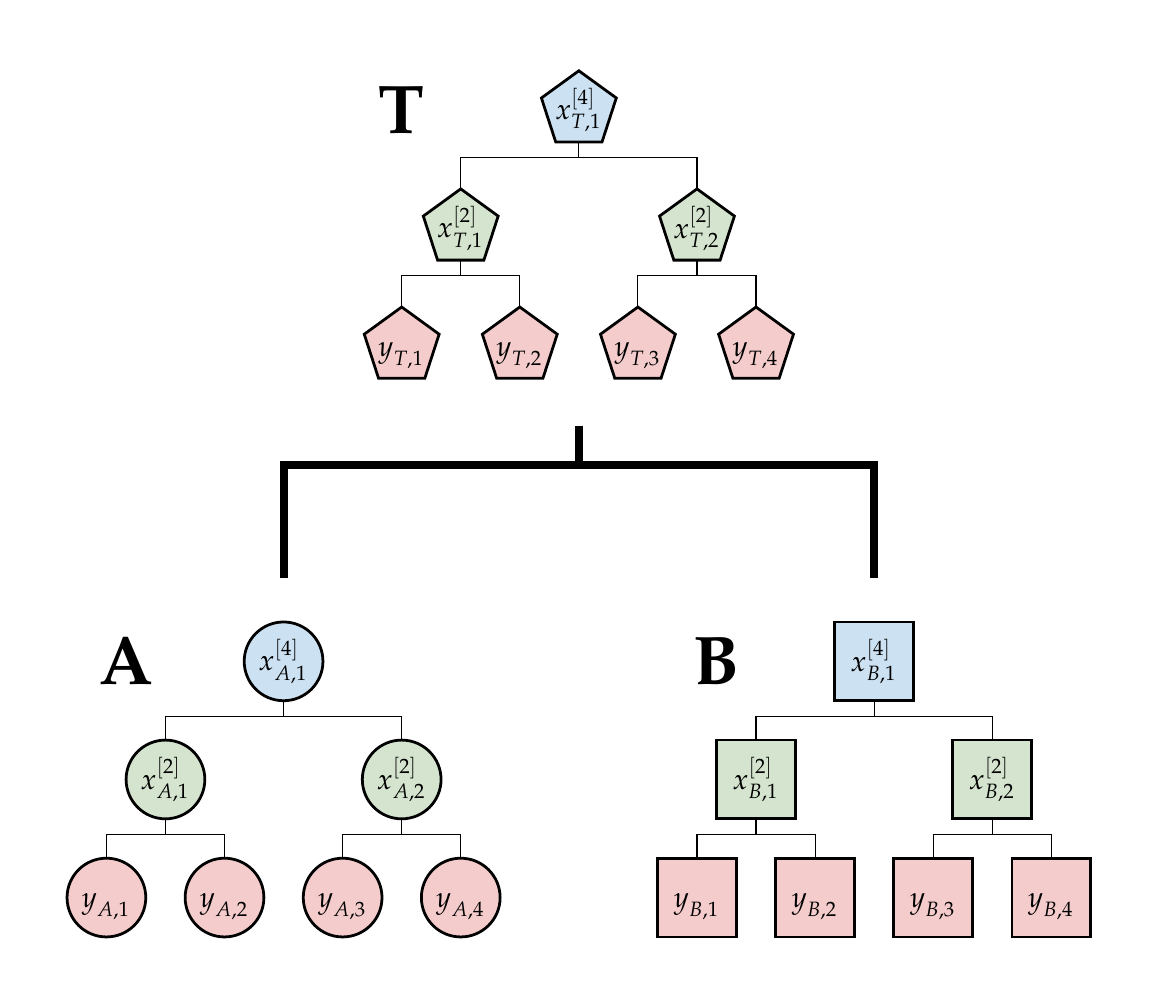
\begin{tikzpicture}[baseline=(current  bounding  box.center),
	every node/.append style={shape=ellipse,
		draw=black},
	minimum width=1.2cm,
	minimum height=1.2cm]

	\Vertex[y = 0, x = 0, label={$y^{\phantom{[1]}}_{A,1}$}, color = newred, opacity = 0.2, size = 1, fontscale=1.5]{5Q1}
	\Vertex[y = 0, x = 1.5, label={$y^{\phantom{[1]}}_{A,2}$}, color = newred, opacity = 0.2, size = 1, fontscale=1.5]{5Q2}
	\Vertex[y = 0, x = 3, label={$y^{\phantom{[1]}}_{A,3}$}, color = newred, opacity = 0.2, size = 1, fontscale=1.5]{5Q3}
	\Vertex[y = 0, x = 4.5, label={$y^{\phantom{[1]}}_{A,4}$}, color = newred, opacity = 0.2, size = 1, fontscale=1.5]{5Q4}
	
	\Vertex[y = 1.5, x = 0.75, label={$x^{[2]}_{A,1}$}, color = avocado, opacity = 0.2, size = 1, shape = circle, fontscale=1.5]{5SA1}
	\Vertex[y = 1.5, x = 3.75,label={$x^{[2]}_{A,2}$}, color = avocado, opacity = 0.2, size = 1,  shape = circle, fontscale=1.5]{5SA2}
	\Vertex[y = 3, x = 2.25,label={$x^{[4]}_{A,1}$}, color = newblue, opacity = 0.2, size = 1,  shape = circle, fontscale=1.5]{5A}
	\relation{0.2}{5Q1}{5SA1};
	\relation{0.2}{5Q2}{5SA1};
	\relation{0.2}{5Q3}{5SA2};
	\relation{0.2}{5Q4}{5SA2};
	\relation{0.2}{5SA1}{5A};
	\relation{0.2}{5SA2}{5A};
	\node[draw=none, align=center] at (0.25,3) {\Huge \color{black} \textbf{A}};
	
	\Vertex[y = 0, x = 7.5, label={$y^{\phantom{[1]}}_{B,1}$}, color = newred, opacity = 0.2, size = 1, shape = rectangle, fontscale=1.5]{6Q1}
	\Vertex[y = 0, x = 9, label={$y^{\phantom{[1]}}_{B,2}$}, color = newred, opacity = 0.2, size = 1, shape = rectangle, fontscale=1.5]{6Q2}
	\Vertex[y = 0, x = 10.5, label={$y^{\phantom{[1]}}_{B,3}$}, color = newred, opacity = 0.2, size = 1, shape = rectangle, fontscale=1.5]{6Q3}
	\Vertex[y = 0, x = 12, label={$y^{\phantom{[1]}}_{B,4}$}, color = newred, opacity = 0.2, size = 1, shape = rectangle, fontscale=1.5]{6Q4}
	\Vertex[y = 1.5, x = 8.25, label={$x^{[2]}_{B,1}$}, color = avocado, opacity = 0.2, size = 1, shape = rectangle, fontscale=1.5]{6SA1}
	\Vertex[y = 1.5, x = 11.25, label={$x^{[2]}_{B,2}$}, color = avocado, opacity = 0.2, size = 1,  shape = rectangle, fontscale=1.5]{6SA2}
	\Vertex[y = 3, x = 9.75, label={$x^{[4]}_{B,1}$}, color = newblue, opacity = 0.2, size = 1,  shape = rectangle, fontscale=1.5]{6A}
	\relation{0.2}{6Q1}{6SA1};
	\relation{0.2}{6Q2}{6SA1};
	\relation{0.2}{6Q3}{6SA2};
	\relation{0.2}{6Q4}{6SA2};
	\relation{0.2}{6SA1}{6A};
	\relation{0.2}{6SA2}{6A};
	\node[draw=none, align=center] at (7.75,3) {\Huge \color{black} \textbf{B}};
	
	\Vertex[y = 7, x = 3.75, label={$y^{\phantom{[1]}}_{T,1}$}, color = newred, opacity = 0.2, size = 1, shape = regular polygon, fontscale=1.5]{7Q1}
	\Vertex[y = 7, x = 5.25, label={$y^{\phantom{[1]}}_{T,2}$}, color = newred, opacity = 0.2, size = 1, shape = regular polygon, fontscale=1.5]{7Q2}
	\Vertex[y = 7, x = 6.75, label={$y^{\phantom{[1]}}_{T,3}$}, color = newred, opacity = 0.2, size = 1, shape = regular polygon, fontscale=1.5]{7Q3}
	\Vertex[y = 7, x = 8.25, label={$y^{\phantom{[1]}}_{T,4}$}, color = newred, opacity = 0.2, size = 1, shape = regular polygon, fontscale=1.5]{7Q4}
	
	\Vertex[y = 8.5, x = 4.5, label={$x^{[2]}_{T,1}$}, color = avocado, opacity = 0.2, size = 1, shape = regular polygon, fontscale=1.5]{7SA1}
	\Vertex[y = 8.5, x = 7.5, label={$x^{[2]}_{T,2}$}, color = avocado, opacity = 0.2, size = 1,  shape = regular polygon, fontscale=1.5]{7SA2}
	\Vertex[y = 10, x = 6, label={$x^{[4]}_{T,1}$}, color = newblue, opacity = 0.2, size = 1,  shape = regular polygon, fontscale=1.5]{7A}
	\relation{0.2}{7Q1}{7SA1};
	\relation{0.2}{7Q2}{7SA1};
	\relation{0.2}{7Q3}{7SA2};
	\relation{0.2}{7Q4}{7SA2};
	\relation{0.2}{7SA1}{7A};
	\relation{0.2}{7SA2}{7A};
	\node[draw=none, align=center] at (3.75,10) {\Huge \color{black} \textbf{T}};
\begin{pgfonlayer}{background} 
	\node[fill=none, line width=3pt, fit={(5Q1) (5Q2) (5Q3) (5Q4) (5SA1) (5SA2) (5A)}, opacity = 0.2, draw = none, shape = rectangle,
	minimum width=6.5cm,
	minimum height=5cm](U1){};	
	\node[fill=none, line width=3pt, fit={(6Q1) (6Q2) (6Q3) (6Q4) (6SA1) (6SA2) (6A)}, opacity = 0.2, draw = none, shape = rectangle,
	minimum width=6.5cm,
	minimum height=5cm](U2){};	
	\node[fill=none, line width=3pt, fit={(7Q1) (7Q2) (7Q3) (7Q4) (7SA1) (7SA2) (7A)}, opacity = 0.2, draw = none, shape = rectangle, 
	minimum width=6.5cm,
	minimum height=5cm
	](T){};	
\end{pgfonlayer}
	\relationBOLD{0.5}{U1}{T};
	\relationBOLD{0.5}{U2}{T};
	\end{tikzpicture}
	}
\end{minipage}\begin{minipage}{0.5\linewidth}
\centering
	\resizebox{\linewidth}{!}{
		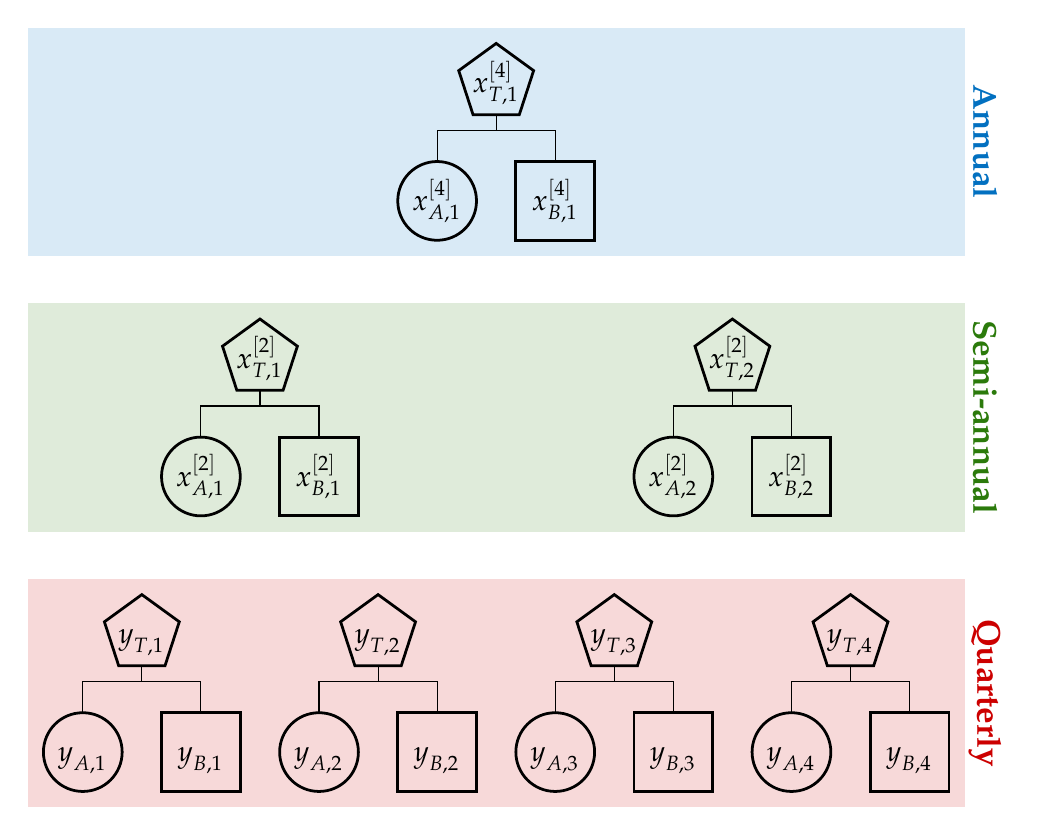
\begin{tikzpicture}[baseline=(current  bounding  box.center),
	every node/.append style={
		draw=black}]

	\Vertex[y = 0, x = 0, label={$y^{\phantom{[1]}}_{A,1}$}, color = none, opacity = 0.2, size = 1, shape = circle, fontscale=1.5]{w1}
	\Vertex[y = 0, x = 1.5, label={$y^{\phantom{[1]}}_{B,1}$}, color = none, opacity = 0.2, size = 1, shape = rectangle, fontscale=1.5]{z1}
	\Vertex[y = 1.5, x = 0.75, label={$y^{\phantom{[1]}}_{T,1}$}, color = none, opacity = 0.2, size = 1, shape = regular polygon, fontscale=1.5]{x1}
	\Vertex[y = 0, x = 3, label={$y^{\phantom{[1]}}_{A,2}$}, color = none, opacity = 0.2, size = 1, shape = circle, fontscale=1.5]{w2}
	\Vertex[y = 0, x = 4.5, label={$y^{\phantom{[1]}}_{B,2}$}, color = none, opacity = 0.2, size = 1, shape = rectangle, fontscale=1.5]{z2}
	\Vertex[y = 1.5, x = 3.75, label={$y^{\phantom{[1]}}_{T,2}$}, color = none, opacity = 0.2, size = 1, shape = regular polygon, fontscale=1.5]{x2}
	
	\Vertex[y = 0, x = 6, label={$y^{\phantom{[1]}}_{A,3}$}, color = none, opacity = 0.2, size = 1, shape = circle, fontscale=1.5]{w3}
	\Vertex[y = 0, x = 7.5, label={$y^{\phantom{[1]}}_{B,3}$}, color = none, opacity = 0.2, size = 1, shape = rectangle, fontscale=1.5]{z3}
	\Vertex[y = 1.5, x = 6.75, label={$y^{\phantom{[1]}}_{T,3}$}, color = none, opacity = 0.2, size = 1, shape = regular polygon, fontscale=1.5]{x3}
	
	\Vertex[y = 0, x = 9, label={$y^{\phantom{[1]}}_{A,4}$}, color = none, opacity = 0.2, size = 1, shape = circle, fontscale=1.5]{w4}
	\Vertex[y = 0, x = 10.5, label={$y^{\phantom{[1]}}_{B,4}$}, color = none, opacity = 0.2, size = 1, shape = rectangle, fontscale=1.5]{z4}
	\Vertex[y = 1.5, x = 9.75, label={$y^{\phantom{[1]}}_{T,4}$}, color = none, opacity = 0.2, size = 1, shape = regular polygon, fontscale=1.5]{x4}
	
	\Vertex[y = 3.5, x = 1.5, label={$x^{[2]}_{A,1}$}, color = none, shape = circle, opacity = 0.2, size = 1, fontscale=1.5]{w12}
	\Vertex[y = 3.5, x = 3, label={$x^{[2]}_{B,1}$}, color = none, shape = rectangle, opacity = 0.2, size = 1, fontscale=1.5]{z12}
	\Vertex[y = 5, x = 2.25, label={$x^{[2]}_{T,1}$}, color = none, shape = regular polygon, opacity = 0.2, size = 1, fontscale=1.5]{x12}
	
	\Vertex[y = 3.5, x = 7.5, label={$x^{[2]}_{A,2}$}, color = none, shape = circle, opacity = 0.2, size = 1, fontscale=1.5]{w22}
	\Vertex[y = 3.5, x = 9, label={$x^{[2]}_{B,2}$}, color = none, shape = rectangle, opacity = 0.2, size = 1, fontscale=1.5]{z22}
	\Vertex[y = 5, x = 8.25, label={$x^{[2]}_{T,2}$}, color = none, shape = regular polygon, opacity = 0.2, size = 1, fontscale=1.5]{x22}
	
	\Vertex[y = 7, x = 4.5, label={$x^{[4]}_{A,1}$}, color = none, shape = circle, opacity = 0.2, size = 1, fontscale=1.5]{w14}
	\Vertex[y = 7, x = 6, label={$x^{[4]}_{B,1}$}, color = none, shape = rectangle, opacity = 0.2, size = 1, fontscale=1.5]{z14}
	\Vertex[y = 8.5, x = 5.25, label={$x^{[4]}_{T,1}$}, color = none, shape = regular polygon, opacity = 0.2, size = 1, fontscale=1.5]{x14}
		
	\relation{0.2}{w1}{x1};
	\relation{0.2}{z1}{x1};
	\relation{0.2}{w2}{x2};
	\relation{0.2}{z2}{x2};
	\relation{0.2}{w3}{x3};
	\relation{0.2}{z3}{x3};
	\relation{0.2}{w4}{x4};
	\relation{0.2}{z4}{x4};
	\relation{0.2}{w12}{x12};
	\relation{0.2}{z12}{x12};
	\relation{0.2}{w22}{x22};
	\relation{0.2}{z22}{x22};
	\relation{0.2}{w14}{x14};
	\relation{0.2}{z14}{x14};
	
	\begin{pgfonlayer}{background}
	\node[draw, color = newred, fill = newred!15, inner sep=2mm, draw = none, label={[name = boot1n, rotate = -90, anchor = center, font = {\large}, yshift = 0.25cm, color = newred] right:{\textbf{Quarterly}}},fit=(w1) (z1) (x1) (w2) (z2) (x2) (w3) (z3) (x3) (w4) (z4) (x4)] (boot1) {};	
	\node[draw, color = avocado, fill = avocado!15, inner sep=2mm, draw = none, yshift = 3.5cm, label={[name = boot2n, rotate = -90, anchor = center, font = {\large}, yshift = 0.25cm, color = avocado] right:{\textbf{Semi-annual}}},fit=(w1) (z1) (x1) (w2) (z2) (x2) (w3) (z3) (x3) (w4) (z4) (x4)] (boot2) {};	
	\node[draw, color = newblue, fill = newblue!15, inner sep=2mm, draw = none, yshift = 7cm, label={[name = boot3n, rotate = -90, anchor = center, font = {\large}, yshift = 0.25cm, color = newblue] right:{\textbf{Annual}}},fit=(w1) (z1) (x1) (w2) (z2) (x2) (w3) (z3) (x3) (w4) (z4) (x4)] (boot3) {};
	\end{pgfonlayer}
	\end{tikzpicture}
}
\end{minipage}}
\end{frame}

\begin{frame}[fragile]{Cross-temporal framework}{\cite{difonzo2023}}
\centering
\vspace{-0.25cm}
\resizebox{\linewidth}{!}{
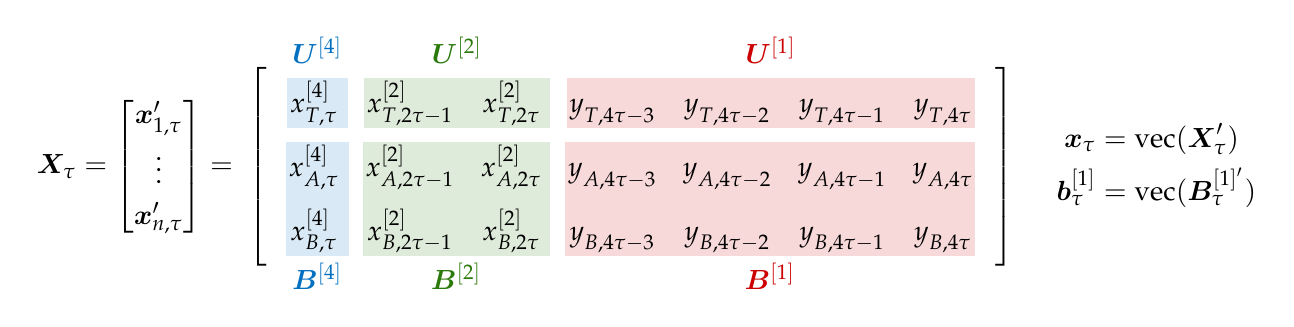
\begin{tikzpicture}[>=latex, Matrix/.style={matrix of nodes, align=center, column sep=1pt, nodes={inner sep=3pt}, row sep=1pt, nodes in empty cells, left delimiter={[}, right delimiter={]}, ampersand replacement=\&}]
\matrix[Matrix] (Mcs){ % Matrix contents
$x^{[4]}_{T,\tau}$ \& $x^{[2]}_{T,2\tau-1}$ \& $x^{[2]}_{T,2\tau}$ \& $y^{\phantom{[1]}}_{T,4\tau-3}$ \& $y^{\phantom{[1]}}_{T,4\tau-2}$ \& $y^{\phantom{[1]}}_{T,4\tau-1}$ \& $y^{\phantom{[1]}}_{T,4\tau}$\\
$x^{[4]}_{A,\tau}$ \& $x^{[2]}_{A,2\tau-1}$ \& $x^{[2]}_{A,2\tau}$ \& $y^{\phantom{[1]}}_{A,4\tau-3}$ \& $y^{\phantom{[1]}}_{A,4\tau-2}$ \& $y^{\phantom{[1]}}_{A,4\tau-1}$ \& $y^{\phantom{[1]}}_{A,4\tau}$\\
$x^{[4]}_{B,\tau}$ \& $x^{[2]}_{B,2\tau-1}$ \& $x^{[2]}_{B,2\tau}$ \& $y^{\phantom{[1]}}_{B,4\tau-3}$ \& $y^{\phantom{[1]}}_{B,4\tau-2}$ \& $y^{\phantom{[1]}}_{B,4\tau-1}$ \& $y^{\phantom{[1]}}_{B,4\tau}$\\
};
\node[left=0cm of Mcs] (pl) {$\Xvet_\tau = \begin{bmatrix}
		\xvet_{1,\tau}' \\[0.1cm]
		\vdots          \\[0.1cm]
		\xvet_{n,\tau}'
	\end{bmatrix} =\quad$};
\node[right=0cm of Mcs] (pl) {$\qquad \begin{aligned}
	\xvet_{\tau} &= \text{vec}(\Xvet_{\tau}') \\
	\bvet_{\tau}^{[1]} &= \text{vec}(\Bvet_{\tau}^{[1]'})
\end{aligned}$};
	\begin{pgfonlayer}{background}
	\node[draw, color = newred, fill = newblue!15, inner sep=-0.75mm, draw = none, label={[anchor = center, font = {\normalsize}, yshift = 0.35cm, color = newblue] above:{$\Uvet^{[4]}$}},fit=(Mcs-1-1)] () {};	
	\node[draw, color = avocado, fill = avocado!15, inner sep=-0.75mm, draw = none, label={[anchor = center, font = {\normalsize}, yshift = 0.35cm, color = avocado] above:{$\Uvet^{[2]}$}},fit=(Mcs-1-2) (Mcs-1-3)] () {};	
	\node[draw, color = newblue, fill = newred!15, inner sep=-0.75mm, draw = none, label={[anchor = center, font = {\normalsize}, yshift = 0.35cm, color = newred] above:{$\Uvet^{[1]}$}},fit=(Mcs-1-4) (Mcs-1-7)] () {};	
	\node[draw, color = newred, fill = newblue!15, inner sep=-0.75mm, draw = none, label={[anchor = center, font = {\normalsize}, yshift = -0.25cm, color = newblue] below:{$\Bvet^{[4]}$}},fit=(Mcs-2-1) (Mcs-3-1)] () {};	
	\node[draw, color = avocado, fill = avocado!15, inner sep=-0.75mm, draw = none, label={[anchor = center, font = {\normalsize}, yshift = -0.25cm, color = avocado] below:{$\Bvet^{[2]}$}},fit=(Mcs-2-2) (Mcs-3-3)] () {};
	\node[draw, color = newblue, fill = newred!15, inner sep=-0.75mm, draw = none, label={[anchor = center, font = {\normalsize}, yshift = -0.25cm, color = newred] below:{$\Bvet^{[1]}$}},fit=(Mcs-2-4) (Mcs-3-7)] () {};
	\end{pgfonlayer}
\end{tikzpicture}}
\vskip0.1cm
\begin{minipage}{0.55\linewidth}
Any cross-temporal matrix may be constructed starting from the one-dimensional equivalents
\begin{itemize}[leftmargin = 1.5cm]
	\item[$\Hvet'\rightarrow$] {\color{avocado}easy} to compute as a function of $\Uvet'$ and of the {\color{newblue}highest time frequency} ($m$)
\end{itemize}
	$$
	\Uvet' \Xvet_{\tau} \Zvet = \Zerovet_{(n_a\times k^\ast)} \; \leftrightarrow \; \Hvet' \xvet_{\tau} = \Zerovet_{[(n_am+nk^\ast)\times1]} 
	$$
\begin{itemize}[leftmargin = 1.5cm]
	\item[$\Fvet\rightarrow$] {\color{avocado}fast} to compute as $\Svet \otimes \Rvet$
\end{itemize}
	$$
	\Xvet_{\tau} = \Svet \Bvet_{\tau}^{[1]} \Rvet' \; \leftrightarrow \; \xvet_{\tau} = \Fvet \bvet_{\tau}^{[1]}
	$$
\end{minipage}\hfill\begin{minipage}{0.4\linewidth}\centering
	\includegraphics[width = \linewidth]{img/code/Untitled6.png}
\begin{minipage}{0.8\linewidth}\tiny
\begin{verbatim}
List of 3
 |-ctf:List of 6
 |  |-Ht     : num [1:36, 1:56] 0 0 0 0 0 0 0 0 0 0 ...
 |  |-Hbrevet: num [1:45, 1:56] 1 0 0 0 0 0 0 0 0 0 ...
 |  |-Hcheckt: num [1:36, 1:56] 1 0 0 0 0 0 0 0 0 0 ...
 |  |-Ccheck : num [1:36, 1:20] 1 1 0 1 0 0 0 1 1 0 ...
 |  |-Scheck : num [1:56, 1:20] 1 1 0 1 0 0 0 1 1 0 ...
 |  |-Fmat   : num [1:56, 1:20] 1 1 0 1 0 0 0 1 1 0 ...
 |-hts:List of 6
 |-thf:List of 8
\end{verbatim}
\end{minipage}
\end{minipage}
\end{frame}

\begin{frame}{Cross-temporal representations}{Two dimensions (\textbf{spatio--temporal}) to capture the complete nature of a multiple time series}
\noindent\makebox[\textwidth][c]{\begin{minipage}[t]{0.5\linewidth}
	\centering
\textbf{Zero-constrained representation}
$$
\Hvet' = \begin{bmatrix}
		(\Zerovet_{(n_a m\times nk^\ast)} ~~ \Ivet_m \otimes \Uvet')\Pvet' \\
		\Ivet_n \otimes \Zvet'
	\end{bmatrix}
$$

\resizebox{0.75\linewidth}{!}{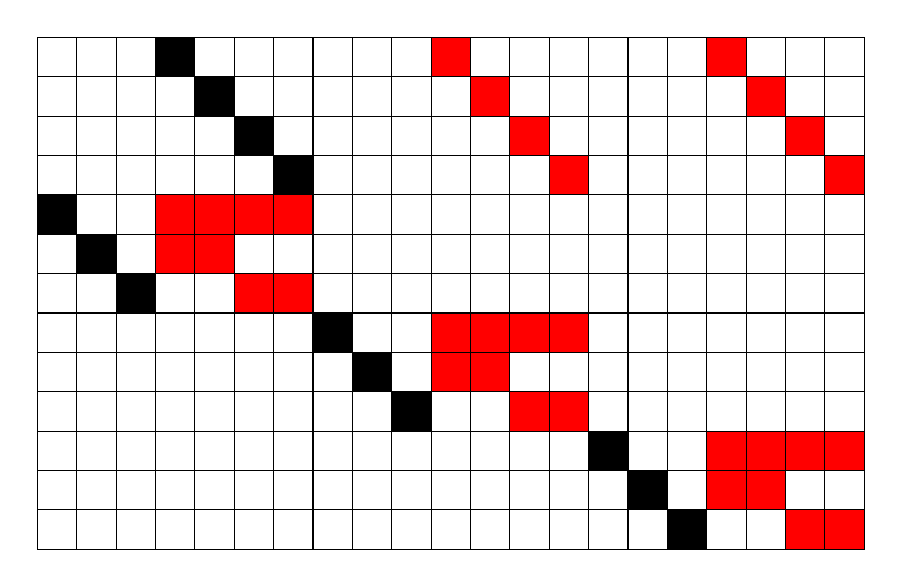
\begin{tikzpicture}
\tikzset{square matrix/.style={
    matrix of nodes, ampersand replacement=\&,
    column sep=-\pgflinewidth, row sep=-\pgflinewidth,
    nodes={draw,
      minimum height=0.5cm,
      anchor=center,
      text width=0.5cm,
      align=center,
      inner sep=0pt,
      font=\tiny
    },
  }
}


\matrix[square matrix](St)
{
|[fill=white]| \& |[fill=white]| \& |[fill=white]| \& |[fill=black]| \& |[fill=white]| \& |[fill=white]| \& |[fill=white]| \& |[fill=white]| \& |[fill=white]| \&  |[fill=white]| \& |[fill=red]| \&  |[fill=white]| \&  |[fill=white]| \&  |[fill=white]| \&  |[fill=white]| \&  |[fill=white]| \&  |[fill=white]| \& |[fill=red]| \&  |[fill=white]| \&  |[fill=white]| \&  |[fill=white]| \\
|[fill=white]| \& |[fill=white]| \& |[fill=white]| \& |[fill=white]| \& |[fill=black]| \& |[fill=white]| \& |[fill=white]| \& |[fill=white]| \& |[fill=white]| \&  |[fill=white]| \&  |[fill=white]| \& |[fill=red]| \&  |[fill=white]| \&  |[fill=white]| \&  |[fill=white]| \&  |[fill=white]| \&  |[fill=white]| \&  |[fill=white]| \& |[fill=red]| \&  |[fill=white]| \&  |[fill=white]| \\
|[fill=white]| \& |[fill=white]| \& |[fill=white]| \& |[fill=white]| \& |[fill=white]| \& |[fill=black]| \& |[fill=white]| \& |[fill=white]| \& |[fill=white]| \&  |[fill=white]| \&  |[fill=white]| \&  |[fill=white]| \& |[fill=red]| \&  |[fill=white]| \&  |[fill=white]| \&  |[fill=white]| \&  |[fill=white]| \&  |[fill=white]| \&  |[fill=white]| \& |[fill=red]| \&  |[fill=white]| \\
|[fill=white]| \& |[fill=white]| \& |[fill=white]| \& |[fill=white]| \& |[fill=white]| \& |[fill=white]| \& |[fill=black]| \& |[fill=white]| \& |[fill=white]| \&  |[fill=white]| \&  |[fill=white]| \&  |[fill=white]| \&  |[fill=white]| \& |[fill=red]| \&  |[fill=white]| \&  |[fill=white]| \&  |[fill=white]| \&  |[fill=white]| \&  |[fill=white]| \&  |[fill=white]| \& |[fill=red]| \\
|[fill=black]| \& |[fill=white]| \& |[fill=white]| \& |[fill=red]| \& |[fill=red]| \& |[fill=red]| \& |[fill=red]| \& |[fill=white]| \& |[fill=white]| \&  |[fill=white]| \&  |[fill=white]| \&  |[fill=white]| \&  |[fill=white]| \&  |[fill=white]| \&  |[fill=white]| \&  |[fill=white]| \&  |[fill=white]| \&  |[fill=white]| \&  |[fill=white]| \&  |[fill=white]| \&  |[fill=white]| \\
|[fill=white]| \& |[fill=black]| \& |[fill=white]| \& |[fill=red]| \& |[fill=red]| \& |[fill=white]| \& |[fill=white]| \& |[fill=white]| \& |[fill=white]| \&  |[fill=white]| \&  |[fill=white]| \&  |[fill=white]| \&  |[fill=white]| \&  |[fill=white]| \&  |[fill=white]| \&  |[fill=white]| \&  |[fill=white]| \&  |[fill=white]| \&  |[fill=white]| \&  |[fill=white]| \&  |[fill=white]| \\
|[fill=white]| \& |[fill=white]| \& |[fill=black]| \& |[fill=white]| \& |[fill=white]| \& |[fill=red]| \& |[fill=red]| \& |[fill=white]| \& |[fill=white]| \&  |[fill=white]| \&  |[fill=white]| \&  |[fill=white]| \&  |[fill=white]| \&  |[fill=white]| \&  |[fill=white]| \&  |[fill=white]| \&  |[fill=white]| \&  |[fill=white]| \&  |[fill=white]| \&  |[fill=white]| \&  |[fill=white]| \\
|[fill=white]| \& |[fill=white]| \& |[fill=white]| \& |[fill=white]| \& |[fill=white]| \& |[fill=white]| \& |[fill=white]| \& |[fill=black]| \& |[fill=white]| \&  |[fill=white]| \& |[fill=red]| \& |[fill=red]| \& |[fill=red]| \& |[fill=red]| \&  |[fill=white]| \&  |[fill=white]| \&  |[fill=white]| \&  |[fill=white]| \&  |[fill=white]| \&  |[fill=white]| \&  |[fill=white]| \\
|[fill=white]| \& |[fill=white]| \& |[fill=white]| \& |[fill=white]| \& |[fill=white]| \& |[fill=white]| \& |[fill=white]| \& |[fill=white]| \& |[fill=black]| \&  |[fill=white]| \& |[fill=red]| \& |[fill=red]| \&  |[fill=white]| \&  |[fill=white]| \&  |[fill=white]| \&  |[fill=white]| \&  |[fill=white]| \&  |[fill=white]| \&  |[fill=white]| \&  |[fill=white]| \&  |[fill=white]| \\
|[fill=white]| \& |[fill=white]| \& |[fill=white]| \& |[fill=white]| \& |[fill=white]| \& |[fill=white]| \& |[fill=white]| \& |[fill=white]| \& |[fill=white]| \&  |[fill=black]| \&  |[fill=white]| \&  |[fill=white]| \& |[fill=red]| \& |[fill=red]| \&  |[fill=white]| \&  |[fill=white]| \&  |[fill=white]| \&  |[fill=white]| \&  |[fill=white]| \&  |[fill=white]| \&  |[fill=white]| \\
|[fill=white]| \& |[fill=white]| \& |[fill=white]| \& |[fill=white]| \& |[fill=white]| \& |[fill=white]| \& |[fill=white]| \& |[fill=white]| \& |[fill=white]| \&  |[fill=white]| \&  |[fill=white]| \&  |[fill=white]| \&  |[fill=white]| \&  |[fill=white]| \&  |[fill=black]| \&  |[fill=white]| \&  |[fill=white]| \& |[fill=red]| \& |[fill=red]| \& |[fill=red]| \& |[fill=red]| \\
|[fill=white]| \& |[fill=white]| \& |[fill=white]| \& |[fill=white]| \& |[fill=white]| \& |[fill=white]| \& |[fill=white]| \& |[fill=white]| \& |[fill=white]| \&  |[fill=white]| \&  |[fill=white]| \&  |[fill=white]| \&  |[fill=white]| \&  |[fill=white]| \&  |[fill=white]| \&  |[fill=black]| \&  |[fill=white]| \& |[fill=red]| \& |[fill=red]| \&  |[fill=white]| \&  |[fill=white]| \\
|[fill=white]| \& |[fill=white]| \& |[fill=white]| \& |[fill=white]| \& |[fill=white]| \& |[fill=white]| \& |[fill=white]| \& |[fill=white]| \& |[fill=white]| \&  |[fill=white]| \&  |[fill=white]| \&  |[fill=white]| \&  |[fill=white]| \&  |[fill=white]| \&  |[fill=white]| \&  |[fill=white]| \&  |[fill=black]| \&  |[fill=white]| \&  |[fill=white]| \& |[fill=red]| \& |[fill=red]| \\
};

\end{tikzpicture}}
$$
\text{where} \quad \Pvet \text{vec}(\Xvet_{\tau}) = \text{vec}(\Xvet_{\tau}')
$$
\end{minipage}\vline\begin{minipage}[t]{0.5\linewidth}
	\centering
\textbf{Structural representation}\\[0.25cm]
\resizebox{0.95\linewidth}{!}{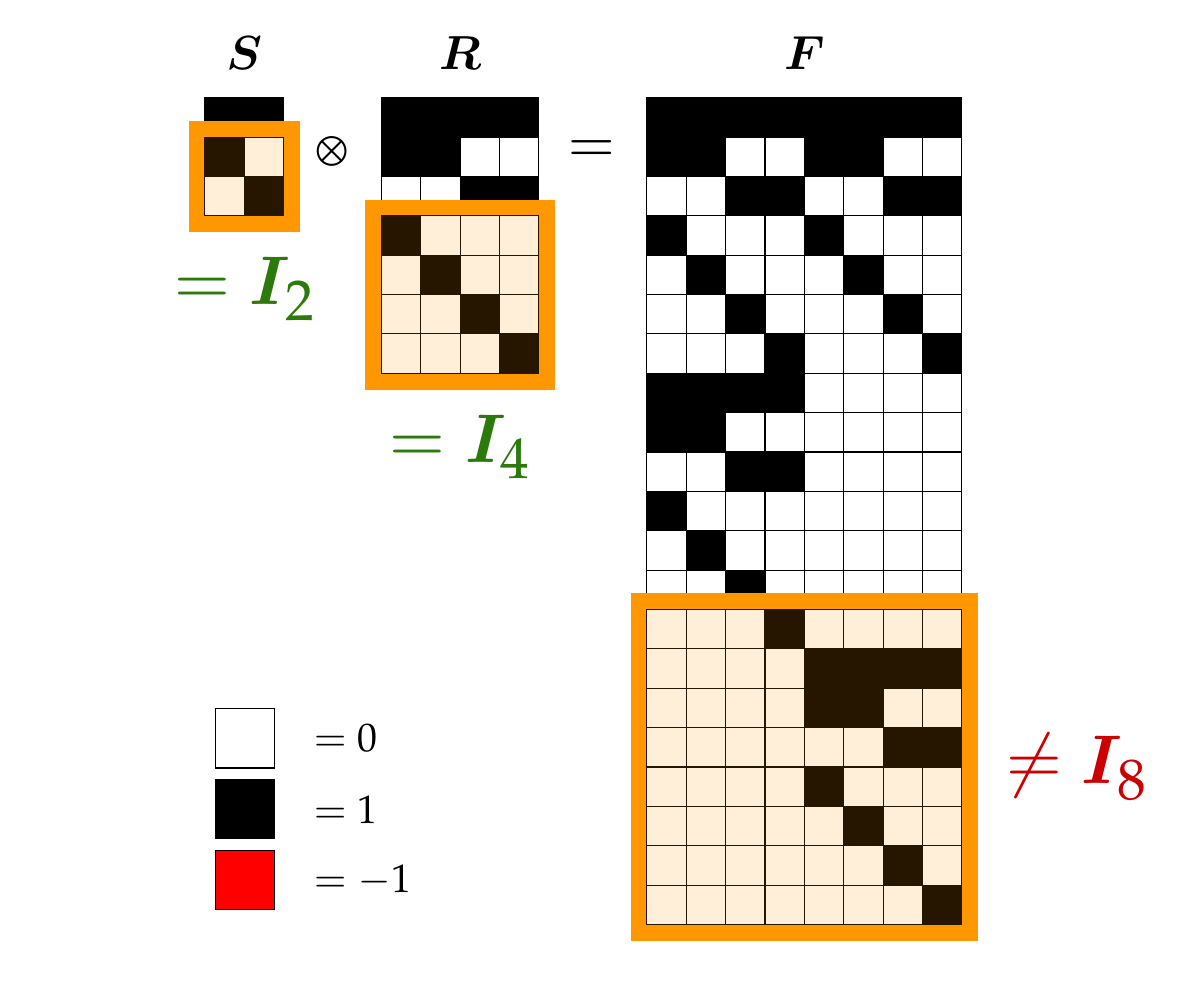
\begin{tikzpicture}
\tikzset{square matrix/.style={
    matrix of nodes,ampersand replacement=\&,
    column sep=-\pgflinewidth, row sep=-\pgflinewidth,
    nodes={draw,
      minimum height=0.5cm,
      anchor=center,
      text width=0.5cm,
      align=center,
      inner sep=0pt,
      font=\scriptsize
    },
  }
}

\node[anchor = center, font = {\LARGE}] (labS) {$\Svet$};
\node[anchor = center, font = {\LARGE}, right= 2cm of labS] (labSte) {$\Rvet$};
\node[anchor = center, font = {\LARGE}, right= 3.6cm of labSte] (labSct) {$\Fvet$};

\node[right= 0.425cm of labS,font=\bfseries, yshift = -1.25cm, font = \large] (kro) {$\bigotimes$};

\node[right= 0.85cm of labSte,font=\bfseries, yshift = -1.25cm, font = \huge] (ugu) {$\mathbf{=}$};

\matrix[square matrix, below = 0.1cm of labS](S)
{
|[fill=black]| \& |[fill=black]| \\
|[fill=black]| \& |[fill=white]| \\
|[fill=white]| \& |[fill=black]| \\
};

\matrix[square matrix, below=of S, yshift = -5cm, xshift = 1.5cm](leg)
{
|[fill=white, minimum height=0.75cm, text width=0.75cm]| \& |[draw=none, align=left, text width=3cm, font = \Large]|$\quad=0$ \\[0.15cm]
|[fill=black, minimum height=0.75cm, text width=0.75cm]| \& |[draw=none, align=left, text width=3cm, font = \Large]|$\quad=1$ \\[0.15cm]
|[fill=red, minimum height=0.75cm, text width=0.75cm]| \& |[draw=none, align=left, text width=3cm, font = \Large]|$\quad=-1$ \\
};

\matrix[square matrix, below = 0.1cm of labSte](K)
{
|[fill=black]| \& |[fill=black]| \& |[fill=black]| \& |[fill=black]| \\
|[fill=black]| \& |[fill=black]| \& |[fill=white]| \& |[fill=white]| \\
|[fill=white]| \& |[fill=white]| \& |[fill=black]| \& |[fill=black]| \\
|[fill=black]| \& |[fill=white]| \& |[fill=white]| \& |[fill=white]| \\
|[fill=white]| \& |[fill=black]| \& |[fill=white]| \& |[fill=white]| \\
|[fill=white]| \& |[fill=white]| \& |[fill=black]| \& |[fill=white]| \\
|[fill=white]| \& |[fill=white]| \& |[fill=white]| \& |[fill=black]| \\
};

\matrix[square matrix, below = 0.1cm of labSct](St)
{
|[fill=black]| \& |[fill=black]| \& |[fill=black]| \& |[fill=black]| \& |[fill=black]| \& |[fill=black]| \& |[fill=black]| \& |[fill=black]| \\
|[fill=black]| \& |[fill=black]| \& |[fill=white]| \& |[fill=white]| \& |[fill=black]| \& |[fill=black]| \& |[fill=white]| \& |[fill=white]| \\
|[fill=white]| \& |[fill=white]| \& |[fill=black]| \& |[fill=black]| \& |[fill=white]| \& |[fill=white]| \& |[fill=black]| \& |[fill=black]| \\
|[fill=black]| \& |[fill=white]| \& |[fill=white]| \& |[fill=white]| \& |[fill=black]| \& |[fill=white]| \& |[fill=white]| \& |[fill=white]| \\
|[fill=white]| \& |[fill=black]| \& |[fill=white]| \& |[fill=white]| \& |[fill=white]| \& |[fill=black]| \& |[fill=white]| \& |[fill=white]| \\
|[fill=white]| \& |[fill=white]| \& |[fill=black]| \& |[fill=white]| \& |[fill=white]| \& |[fill=white]| \& |[fill=black]| \& |[fill=white]| \\
|[fill=white]| \& |[fill=white]| \& |[fill=white]| \& |[fill=black]| \& |[fill=white]| \& |[fill=white]| \& |[fill=white]| \& |[fill=black]| \\
|[fill=black]| \& |[fill=black]| \& |[fill=black]| \& |[fill=black]| \& |[fill=white]| \& |[fill=white]| \& |[fill=white]| \& |[fill=white]| \\
|[fill=black]| \& |[fill=black]| \& |[fill=white]| \& |[fill=white]| \& |[fill=white]| \& |[fill=white]| \& |[fill=white]| \& |[fill=white]| \\
|[fill=white]| \& |[fill=white]| \& |[fill=black]| \& |[fill=black]| \& |[fill=white]| \& |[fill=white]| \& |[fill=white]| \& |[fill=white]| \\
|[fill=black]| \& |[fill=white]| \& |[fill=white]| \& |[fill=white]| \& |[fill=white]| \& |[fill=white]| \& |[fill=white]| \& |[fill=white]| \\
|[fill=white]| \& |[fill=black]| \& |[fill=white]| \& |[fill=white]| \& |[fill=white]| \& |[fill=white]| \& |[fill=white]| \& |[fill=white]| \\
|[fill=white]| \& |[fill=white]| \& |[fill=black]| \& |[fill=white]| \& |[fill=white]| \& |[fill=white]| \& |[fill=white]| \& |[fill=white]| \\
|[fill=white]| \& |[fill=white]| \& |[fill=white]| \& |[fill=black]| \& |[fill=white]| \& |[fill=white]| \& |[fill=white]| \& |[fill=white]| \\
|[fill=white]| \& |[fill=white]| \& |[fill=white]| \& |[fill=white]| \& |[fill=black]| \& |[fill=black]| \& |[fill=black]| \& |[fill=black]| \\
|[fill=white]| \& |[fill=white]| \& |[fill=white]| \& |[fill=white]| \& |[fill=black]| \& |[fill=black]| \& |[fill=white]| \& |[fill=white]| \\
|[fill=white]| \& |[fill=white]| \& |[fill=white]| \& |[fill=white]| \& |[fill=white]| \& |[fill=white]| \& |[fill=black]| \& |[fill=black]| \\
|[fill=white]| \& |[fill=white]| \& |[fill=white]| \& |[fill=white]| \& |[fill=black]| \& |[fill=white]| \& |[fill=white]| \& |[fill=white]| \\
|[fill=white]| \& |[fill=white]| \& |[fill=white]| \& |[fill=white]| \& |[fill=white]| \& |[fill=black]| \& |[fill=white]| \& |[fill=white]| \\
|[fill=white]| \& |[fill=white]| \& |[fill=white]| \& |[fill=white]| \& |[fill=white]| \& |[fill=white]| \& |[fill=black]| \& |[fill=white]| \\
|[fill=white]| \& |[fill=white]| \& |[fill=white]| \& |[fill=white]| \& |[fill=white]| \& |[fill=white]| \& |[fill=white]| \& |[fill=black]| \\
|[draw=none]| \& |[draw=none]| \& |[draw=none]| \& |[draw=none]| \& |[draw=none]| \& |[draw=none]| \& |[draw=none]| \& |[draw=none]| \\
};

\node[fit=(S-2-1.north west)(S-3-2.south east), draw = DarkOrange, line width=2mm, fill = DarkOrange, fill opacity = 0.15, inner sep = 1mm, label={[font=\Huge,text=avocado, yshift = -2mm]below:{$=\Ivet_2$}}]{};
\node[fit=(K-4-1.north west)(K-7-4.south east), draw = DarkOrange, line width=2mm, fill = DarkOrange, fill opacity = 0.15, inner sep = 1mm, label={[font=\Huge,text=avocado, yshift = -2mm]below:{$=\Ivet_4$}}]{};
\node[fit=(St-14-1.north west)(St-21-8.south east), draw = DarkOrange, line width=2mm, fill = DarkOrange, fill opacity = 0.15, inner sep = 1mm, label={[font=\Huge,text=newred, xshift = 2mm]right:{$\neq\Ivet_8$}}]{};
\phantom{\node[fit=(S-2-1.north west)(S-3-2.south east), draw = DarkOrange, line width=2mm, fill = DarkOrange, fill opacity = 0.15, inner sep = 1mm, label={[font=\Huge,text=avocado, yshift = -2mm]left:{$=\Ivet_2$}}]{};}
\end{tikzpicture}}
\end{minipage}}
\end{frame}

\section{Point forecast reconciliation (cross-temporal framework)}

\begin{frame}{Point forecast reconciliation}{\cite{wickramasuriya2019, panagiotelis2021}}\centering
\begin{minipage}{0.65\linewidth}
	\begin{alertblock}{Definition}
Forecast reconciliation aims to adjust the base forecast $\widehat{\xvet}_{h}$ via a mapping $\psi: \mathbb{R}^{n(m+k^\ast)} \rightarrow \mathfrak{s}$ such that $$\widetilde{\xvet}_{h} = \psi\left(\widehat{\xvet}_{h}\right),$$ where $\widetilde{\xvet}_{h} \in \mathfrak{s}$ is the vector of the reconciled forecasts
\end{alertblock}
\end{minipage}\hfill\begin{minipage}{0.3\linewidth}
	\resizebox{\linewidth}{!}{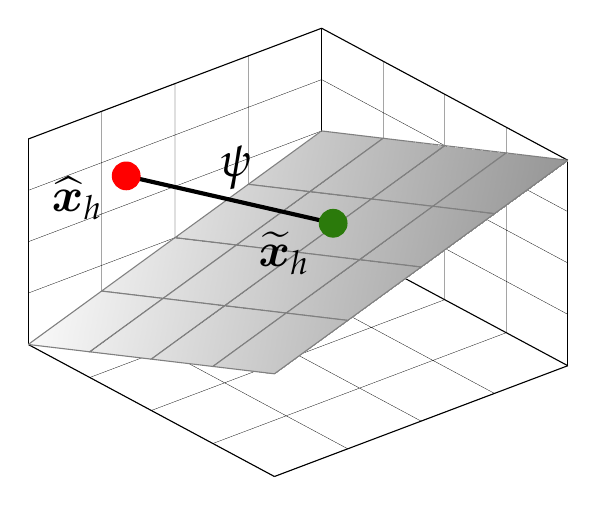
\begin{tikzpicture}
\begin{axis}[view = {50}{40},
    xmax = 5,
    xmin = -5,
    ymax = 5, 
    ymin = -5, 
    zmax = 10, 
    zmin = -10,
    xtick = \empty,
    ytick = \empty,
    ztick = \empty,
    grid]

\addplot3 [mark = .,color = black,line width=0.1pt] coordinates {
    (-2.5,-5,-10)
    (-2.5,5,-10)
    (-2.5,5,10)
    (0,5,10)
    (0,5,-10)
    (0,-5,-10)
    (2.5,-5,-10)
    (2.5,5,-10)
    (2.5,5,10)
    (5,5,10)
    (5,5,5)
    (-5,5,5)
    (-5,-5,5)
    (-5,-5,0)
    (-5,5,0)
    (5,5,0)
    (5,5,-5)
    (-5,5,-5)
    (-5,-5,-5)
    (-5,-5,-10)
    (5,-5,-10)
    (5,-2.5,-10)
    (-5,-2.5,-10)
    (-5,-2.5,10)
    (-5,0,10)
    (-5,0,-10)
    (5,0,-10)
    (5,2.5,-10)
    (-5,2.5,-10)
    (-5,2.5,10)
};

\addplot3 [
    domain=-5:5,
    domain y = -5:5,
    samples = 5,
    surf,
    colormap= {blueblack}{color=(VeryLightGray) color=(LightGray)},
    shader = faceted interp,
    faceted color = gray] {x + y};

\addplot3 [
    mark         = .,
    color = black,
    line width=1.5pt
  ] coordinates 
{
    (-4,-2.5,5)
    (-0.17,1.34,1.17)
};

\addplot3 [
    mark options = {color=red},
    mark size=5pt,
    mark         = *
  ] coordinates 
{
    (-4,-2.5,5)
};

\addplot3 [
    mark options = {color=avocado},
    mark size=5pt,
    mark         = *
  ] coordinates 
{
    (-0.17,1.34,1.17)
};
\node at (axis cs:-2,1.2,-4) {\LARGE$\widetilde{\xvet}_h$};
\node at (axis cs:-4.5,-3.75,3.5) {\LARGE$\widehat{\xvet}_h$};
\node at (axis cs:-2.5,0,5) {\LARGE$\psi$};
\end{axis}
\end{tikzpicture}}
\end{minipage}
\begin{tikzpicture}[Deco/.style = {postaction = {pattern = {
Lines[angle=45, distance=3mm,  line width=1.5mm]%
}, pattern color = newred}}]
\begin{scope}[fill opacity = 0.25]
\draw[fill = newblue, color = newblue] (0, 0) ellipse (2cm and 1cm);
\draw[fill = avocado, color = avocado] (2, 0) ellipse (2cm and 1cm);
\end{scope}
\begin{scope}
	\clip (0, 0) ellipse (2cm and 1cm);
	\fill[Deco, fill = none] (2, 0) ellipse (2cm and 1cm);
\end{scope}
\node[text width = 3cm, align = center, color = newblue] at (-4.5, 0) (a){\Large$\mathfrak{s}_{cs}$ \\ {\footnotesize cross-sectional \textit{coherent} \\[-0.025cm] \textit{subspace} spanned by \\[-0.1cm] the columns of $\Svet$}};
\node[right = -0.25mm of a, color = newblue] (){\faArrowLeft};
\node[text width = 3cm, align = center, color = avocado] at (6.5, 0) (b){\Large$\mathfrak{s}_{te}$ \\ {\footnotesize temporal \textit{coherent} \\[-0.025cm] \textit{subspace} spanned by \\[-0.1cm] the columns of $\Rvet$}};
\node[left = -0.25mm of b, color = avocado] (){\faArrowRight};
\node[text width = 12cm, align = center, color = newred] at (1, -1.75) (c){\Large$\mathfrak{s}$ {\footnotesize cross-temporal \textit{coherent} \textit{subspace} spanned by the columns of $\Fvet = \Svet \otimes \Rvet$}};
\node[above = -0.5mm of c, color = newred] (){\faArrowDown};
\end{tikzpicture}
\end{frame}

\begin{frame}[label = {cap:opt}]{Optimal forecast reconciliation}
\centering
\begin{tabular}{M{0.25\linewidth}M{0.25\linewidth}cM{0.25\linewidth}}
	{\color{newred}Base forecasts} & Target & & {\color{avocado}Reconciled forecasts} \\
	{\color{newred}$\Hvet'\widehat{\xvet}_h\neq \Zerovet$} & $\Hvet'\xvet_h = \Zerovet$ & $\bm{\rightarrow}$ & {\color{avocado}$\Hvet'\widetilde{\xvet}_h = \Zerovet$}
\end{tabular}	
\begin{enumerate}
	\item Forecast \textbf{all series at all levels} of aggregation (using e.g. ARIMA, ETS, VAR ...) $\rightarrow$ {\color{newred}base forecasts}\\[0.2cm]
	\item Make the base forecasts \textbf{coherent} %using least squares 
	$\rightarrow$ {\color{avocado}reconciled forecasts}
	\begin{itemize}[nosep, topsep = 0.1cm]
		\item[\faPlay] \hyperlink{app:proj}{\textbf{Projection approach}} \citep{byron1978, byron1979}\\[-0.55cm]
		$$
		\begin{array}{c}
			\displaystyle\argmin_{\xvet_h}\;\; (\widehat{\xvet}_h-\xvet_h)'\Omegavet_{ct}^{-1}(\widehat{\xvet}_h-\xvet_h)\\[0.1cm]
			\text{s.t.} \quad \Hvet'\xvet_h = \Zerovet
		\end{array}\Rightarrow \quad \widetilde{\xvet}_h =\left[\Ivet - \Omegavet_{ct}\Hvet\left({\Hvet'}\Omegavet_{ct}\Hvet\right)^{-1}\Hvet'\right]\widehat{\xvet}_h = \psi\left(\widehat{\xvet}_h\right)\vspace{-0.25cm}
		$$
		\item[\faPlay] \hyperlink{app:strc}{\textbf{Structural approach}} \citep[cross-temporal extension]{wickramasuriya2019}\\[-0.2cm]
		$$
		\begin{array}{c}
			\displaystyle\min_{\Gvet}\;\; \mbox{tr}\left(\Fvet\Gvet\Omegavet_{ct}\Gvet'\Svet'_{ct}\right)\\[0.1cm]
			\text{s.t.} \quad \Fvet\Gvet\Fvet = \Fvet
		\end{array}\Rightarrow \quad \widetilde{\xvet}_h =\Fvet\underbrace{(\Fvet' \Omegavet_{ct}^{-1}\Fvet)^{-1} \Fvet'\Omegavet_{ct}^{-1}}_{\Gvet}\widehat{\xvet}_h = \psi\left(\widehat{\xvet}_h\right)
		$$
\end{itemize}
\end{enumerate}
\begin{itemize}
	\item[\faThumbtack] The formulation of $\text{Var}(\widehat{\xvet}_h -\xvet_h)$ is conceptually {\color{newred}complex}; in practice, \hyperlink{app:cov}{\ul{approximate forms}} of $\text{Var}(\widehat{\xvet}_h -\xvet_h) \approx \Omegavet_{ct}$ are used, possibly using in-sample residuals
	\end{itemize}
\end{frame}

\begin{frame}{Projection vs structural approach}{\texttt{FoReco 0.2.6} - cross-sectional ols reconciliation - $time$ in seconds}
	\centering
	\begin{minipage}{0.625\linewidth}
	\includegraphics[width = 0.9\linewidth]{img/time.pdf}
	\end{minipage}\begin{minipage}{0.35\linewidth}
	Two main factors:
	\begin{itemize}
		\item dimensions 
		\begin{itemize}
			\item[{\color{avocado}cs:}] {\color{avocado}$n_a$, $n_b$}
			\item[te:] $\mathcal{K}$
			\item[ct:] $n_a$, $n_b$, $\mathcal{K}$
		\end{itemize}
		\item {\color{newred}Computational cost of $\Omegavet_{ct}^{-1}$}
	\end{itemize}
	\vskip0.5cm
	\hrule
	\vskip0.5cm
	$$
	value = \frac{time_{\text{strc}}-time_{\text{proj}}}{time_{\text{strc}}+time_{\text{proj}}}
	$$
		\begin{itemize}[leftmargin=*]
			\item[\faArrowDown] $value < 0 \Rightarrow$ structural is faster
			\item[\faArrowUp] $value > 0 \Rightarrow$ projection is faster
		\end{itemize}
	\end{minipage}
\end{frame}

\section{Probabilistic forecast reconciliation (cross-temporal framework)}

\begin{frame}{Probabilistic forecast reconciliation}{Starting point}
\centering
	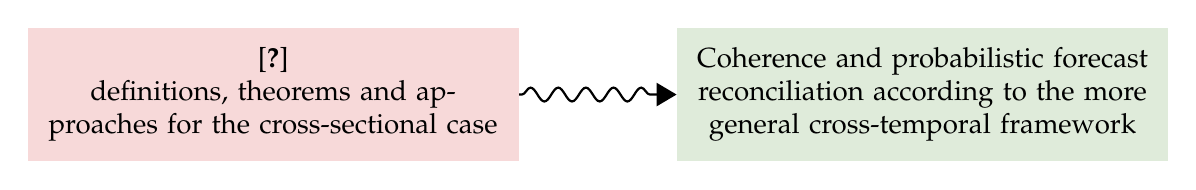
\begin{tikzpicture}
		\node[fill = newred!15, text width = 6cm, align = center, inner ysep = 0.25cm] (cs){\cite{panagiotelis2023} \\
		definitions, theorems and approaches for the cross-sectional case};
		\node[fill = avocado!15, text width = 6cm, align = center, right=2cm of cs, inner ysep = 0.25cm] (ct){Coherence and probabilistic forecast reconciliation according to the more general cross-temporal framework};
		\draw[-{Triangle[scale=1.5]}, decorate, decoration={snake,pre length=1pt,post length=8pt}, thick, shorten >= 0pt] (cs) -- (ct);
	\end{tikzpicture}
	\begin{itemize}
		\item[\faThumbtack] A generalized probabilistic cross-temporal framework for {\color{newred}\textbf{count data}} can be obtained following the cross-sectional work of \cite{corani2022} $\rightarrow$ however, we only focus on the {\color{avocado}\textbf{continuous case}}
	\end{itemize}
	\begin{exampleblock}{Thm: Cross-temporal Reconciled Samples}\centering
	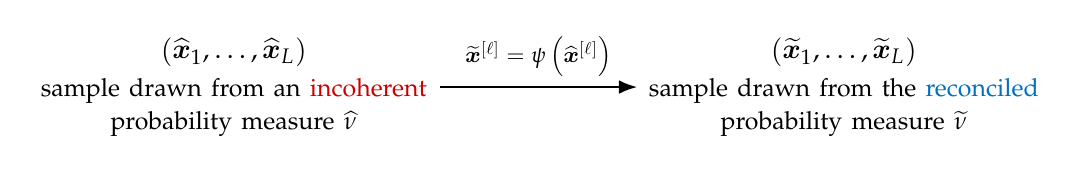
\begin{tikzpicture}[baseline=(current  bounding  box.center)]
	\node[text width=5cm, align=center] (A){$\left(\widehat{\xvet}_1, \dots, \widehat{\xvet}_L\right)$ \\[0.25em] {\small sample drawn from an {\color{newred}incoherent} \\ probability measure $\widehat{\nu}$}};
	\node[text width=5cm, align=center, right=2.5cm of A] (B){$\left(\widetilde{\xvet}_1, \dots, \widetilde{\xvet}_L\right)$ \\[0.25em] {\small sample drawn from the {\color{newblue}reconciled} \\probability measure $\widetilde{\nu}$}};
	\draw [thick, -{Latex}] (A) -- (B) node[midway,above] {\footnotesize $\widetilde{\xvet}^{[\ell]}=\psi\left(\widehat{\xvet}^{[\ell]}\right)$};
\end{tikzpicture}
	\end{exampleblock}
\end{frame}

\begin{frame}[label = {cap:samples}]{A parametric gaussian approach}{Base forecasts sample paths \citep{panagiotelis2023, wickramasuriya2021b}}
\hspace{1cm}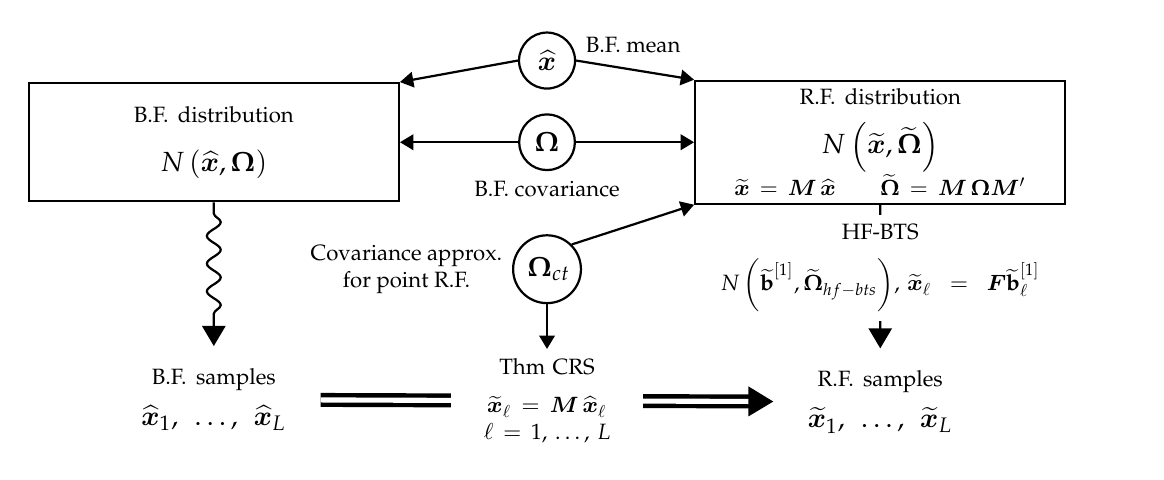
\begin{tikzpicture}
\node[draw, thick, inner sep=1mm, minimum width = 1cm, text width=4.5cm, minimum height = 1.5cm, text centered] (dist) {{\footnotesize R.F. distribution} \\[0.2cm]
$N\left(\widetilde{\xvet}, \widetilde{\Omegavet} \right)$\\
{\footnotesize $\widetilde{\xvet} = \Mvet\,\widehat{\xvet}\qquad \widetilde{\Omegavet} = \Mvet\,\Omegavet\Mvet'$}};

\node[draw, thick, circle, inner sep=1mm, text width=0.35cm, text centered, minimum width = 0.5cm, minimum height = 0.5cm, left= 1.5cm of dist, label={[align=center, font=\footnotesize]below:{B.F. covariance}}] (cov) {$\Omegavet$};

\node[draw, thick, inner sep=1mm, minimum width = 1cm, text width=4.5cm, minimum height = 1.5cm, text centered, left= 1.5cm of cov] (dist2) {{\footnotesize B.F. distribution} \\[0.2cm] $N\left(\widehat{\xvet}, \Omegavet\right)$};

\node[draw, thick, circle, inner sep=1mm, text width=0.5cm, text centered, minimum width = 0.5cm, minimum height = 0.5cm, below = 0.8cm of cov, label={[align=center, font=\footnotesize]left:{Covariance approx. \\for point R.F.}}] (covapprx) {$\Omegavet_{ct}$};

\node[draw, thick, circle, inner sep=1mm, text width=0.35cm, text centered, minimum width = 0.5cm, minimum height = 0.5cm, above = 0.3cm of cov, label={[yshift = 0.2cm]right:{\footnotesize B.F. mean}}] (mean) {$\widehat{\xvet}$};

\node[inner sep=1mm, minimum width = 1cm, text width=2.5cm, text centered, below= 2cm of dist2] (sim_base) {{\footnotesize B.F. samples} \\[0.1cm] $\widehat{\xvet}_{1}, \;\dots, \;\widehat{\xvet}_{L}$};

\node[inner sep=1mm, minimum width = 1cm, text width=2.5cm, text centered, below= 2cm of dist] (sim_reco) {{\footnotesize R.F. samples} \\[0.1cm] $\widetilde{\xvet}_{1}, \;\dots, \;\widetilde{\xvet}_{L}$};

\draw[-{Triangle[scale=1]}, decorate, thick] (mean.east) -- (dist.north west);
\draw[-{Triangle[scale=1]}, decorate, thick] (cov) -- (dist);
\draw[-{Triangle[scale=1]}, decorate, thick] (mean.west) -- (dist2.north east);
\draw[-{Triangle[scale=1]}, decorate, thick] (cov) -- (dist2);

\draw[-{Triangle[scale=0.5]}, decorate, ultra thick, double, double distance=0.65mm] (sim_base) -- (sim_reco);

\draw[draw=none,fill=none] (sim_base) -- node[fill=white, anchor=center, pos=0.5,font = \footnotesize, text width = 2.2cm, text centered] (nodemid) {Thm CRS \\[0.15cm] $\widetilde{\xvet}_{\ell} = \Mvet\,\widehat{\xvet}_{\ell}$ \\ $\ell = 1,\, \dots,\, L$} (sim_reco);

\draw[-{Triangle[scale=1]}, decorate, thick] (covapprx.south) -- (nodemid.north);

\draw [-{Triangle[scale=1.5]}, decorate, decoration={snake,pre length=4pt,post length=15pt}, thick, shorten >= 5pt] (dist2) -- (sim_base);

\draw [-{Triangle[scale=1.5]}, decorate, decoration={snake,pre length=4pt,post length=15pt}, thick, shorten >= 5pt] (dist) -- (sim_reco)  node[draw=none, midway, font = \footnotesize, text width = 6.25cm, text centered, fill = white, yshift = 0.2cm] {HF-BTS\\[0.2cm]$N\left(\widetilde{\textbf{b}}^{[1]}, \widetilde{\Omegavet}_{hf-bts} \right)$, $\widetilde{\xvet}_{\ell}=\Fvet \widetilde{\textbf{b}}^{[1]}_{\ell}$};
\draw[-{Triangle[scale=1]}, decorate, thick] (covapprx.north east) -- (dist.south west);
\end{tikzpicture}

\begin{itemize}
	\item \hyperlink{app:ctcov}{\ul{$\Omegavet$ and $\Omegavet_{ct}$ estimates} may consider {\color{avocado}cross-sectional and/or temporal dimensions}} (G, H, B, HB)
	\item Using in-sample residuals is {\color{newred}challenging} \faArrowRight \; \hyperlink{app:multi}{\textbf{\color{avocado}multi-step residuals}}
\end{itemize}
\end{frame}

\begin{frame}{A non-parametric bootstrap approach}{Base forecasts sample paths \citep{panagiotelis2023}}
	\begin{itemize}
	\item {\color{newblue}Analytical expressions} for the base and reconciled forecast distributions are {\color{newred}challenging} and parametric assumptions can be {\color{newred}restrictive and unrealistic}
		\item \textbf{Joint (block) Bootstrap:} simulate future {\color{newred}base sample} paths from all models using {\color{avocado}bootstrapped residuals}, then \textbf{reconcile} them to obtain {\color{avocado}coherent sample paths}
		$$
		\widehat{\xvet}_{i,\ell}^{[k]} = f_i(\mathcal{M}_i, \widehat{\evet}_{i, \tau}^{[k]}) 
		$$
		\item Need to generate samples that preserve \textbf{\color{avocado}cross-temporal} relationships
		\item[{\faIcon[regular]{lightbulb}}] \textbf{Idea}
		\begin{enumerate}
			\item sampling the index time $\tau$ from the {\color{avocado}most temporally aggregated level}
			\item using it to determine the \textbf{indices for all the other levels}
		\end{enumerate}
	\vskip0.25cm
	\item[\faPlus] {\color{avocado}Easily scalable} in order to utilize multiple computing power simultaneously for each series
		\item[\faPlus]  
		 Take into account the  {\color{avocado}dependence between the different levels of temporal aggregation} and not only the {\color{avocado} cross-sectional dependencies}
	\end{itemize}
\end{frame}

\begin{frame}{Example of bootstrapped residuals}{$T = A + B$, 16 quarterly data: the green, blue, red and black colors correspond, respectively, to years 1, 2, 3 and 4.}
\centering
	\begin{tikzpicture}
\matrix (e1) [matrix of nodes,ampersand replacement=\&,row sep=0cm,column sep=0cm, nodes= {rectangle, fill=white, inner sep = 1pt, font = {\fontsize{7}{6}\selectfont}, minimum width=1em, minimum height=1em,anchor=center}, label={[xshift = 0.5em, yshift = -2mm]above:{\footnotesize$\widehat{\textbf{E}}^{[1]}$}}]
{
$T$ \& \pgfuseimage{ngreen2} \& \pgfuseimage{ngreen2} \& \pgfuseimage{ngreen2} \& \pgfuseimage{ngreen2} \& \pgfuseimage{nblue2} \& \pgfuseimage{nblue2}  \& \pgfuseimage{nblue2} \& \pgfuseimage{nblue2} \& \pgfuseimage{nred2} \& \pgfuseimage{nred2} \& \pgfuseimage{nred2} \& \pgfuseimage{nred2} \& \pgfuseimage{nblack2} \& \pgfuseimage{nblack2} \& \pgfuseimage{nblack2} \& \pgfuseimage{nblack2}\\
$A$ \& \pgfuseimage{ngreen2} \& \pgfuseimage{ngreen2} \& \pgfuseimage{ngreen2} \& \pgfuseimage{ngreen2} \& \pgfuseimage{nblue2} \& \pgfuseimage{nblue2}  \& \pgfuseimage{nblue2} \& \pgfuseimage{nblue2} \& \pgfuseimage{nred2} \& \pgfuseimage{nred2} \& \pgfuseimage{nred2} \& \pgfuseimage{nred2} \& \pgfuseimage{nblack2} \& \pgfuseimage{nblack2} \& \pgfuseimage{nblack2} \& \pgfuseimage{nblack2}\\
$B$ \& \pgfuseimage{ngreen2} \& \pgfuseimage{ngreen2} \& \pgfuseimage{ngreen2} \& \pgfuseimage{ngreen2} \& \pgfuseimage{nblue2} \& \pgfuseimage{nblue2}  \& \pgfuseimage{nblue2} \& \pgfuseimage{nblue2} \& \pgfuseimage{nred2} \& \pgfuseimage{nred2} \& \pgfuseimage{nred2} \& \pgfuseimage{nred2} \& \pgfuseimage{nblack2} \& \pgfuseimage{nblack2} \& \pgfuseimage{nblack2} \& \pgfuseimage{nblack2}\\
\& 1 \& 2 \& 3 \& 4 \& 5 \& 6 \& 7 \& 8 \& 9 \& 10 \& 11 \& 12 \& 13 \& 14 \& 15 \& 16 \\
};
\draw[decorate,thick, decoration={brace, mirror, amplitude=5pt,raise=-1pt}] (e1-4-2.south west) -- (e1-4-17.south east) node[midway, font = {\fontsize{7}{6}\selectfont}, yshift = -1em]{Quarterly, $t = 1,\dots,16$};

\matrix (ek) [above= 10mm of e1.north east, anchor=south east, matrix of nodes,ampersand replacement=\&,row sep=0cm,column sep=0cm, nodes= {rectangle, fill=white, inner sep = 1pt, font = {\fontsize{7}{6}\selectfont}, minimum width=1em, minimum height=1em,anchor=center}, label={[xshift = 0.5em, yshift = -2mm]above:{\footnotesize$\widehat{\textbf{E}}^{[2]}$}}]
{
$T$ \& \pgfuseimage{ngreen2} \& \pgfuseimage{ngreen2} \& \pgfuseimage{nblue2} \& \pgfuseimage{nblue2} \& \pgfuseimage{nred2} \& \pgfuseimage{nred2} \& \pgfuseimage{nblack2} \& \pgfuseimage{nblack2}\\
$A$ \& \pgfuseimage{ngreen2} \& \pgfuseimage{ngreen2} \& \pgfuseimage{nblue2} \& \pgfuseimage{nblue2} \& \pgfuseimage{nred2} \& \pgfuseimage{nred2} \& \pgfuseimage{nblack2} \& \pgfuseimage{nblack2}\\
$B$ \& \pgfuseimage{ngreen2} \& \pgfuseimage{ngreen2} \& \pgfuseimage{nblue2} \& \pgfuseimage{nblue2} \& \pgfuseimage{nred2} \& \pgfuseimage{nred2} \& \pgfuseimage{nblack2} \& \pgfuseimage{nblack2}\\
\& 1 \& 2 \& 3 \& 4 \& 5 \& 6 \& 7 \& 8 \\
};
\draw[decorate,thick, decoration={brace, mirror, amplitude=5pt,raise=-1pt}] (ek-4-2.south west) -- (ek-4-9.south east) node[midway, font = {\fontsize{7}{6}\selectfont}, yshift = -1em]{Semi-annual, $j = 1,\dots,8$};

\matrix (em) [above= 10mm of e1.north west, anchor=south west, matrix of nodes,ampersand replacement=\&,row sep=0cm,column sep=0cm, nodes= {rectangle, fill=white, inner sep = 1pt, font = {\fontsize{7}{6}\selectfont}, minimum width=1em, minimum height=1em,anchor=center}, label={[xshift = 0.5em, yshift = -2mm]above:{\footnotesize$\widehat{\textbf{E}}^{[4]}$}}]
{
$T$ \& \pgfuseimage{ngreen2} \& \pgfuseimage{nblue2} \& \pgfuseimage{nred2} \& \pgfuseimage{nblack2}\\
$A$ \& \pgfuseimage{ngreen2} \& \pgfuseimage{nblue2} \& \pgfuseimage{nred2} \& \pgfuseimage{nblack2}\\
$B$ \& \pgfuseimage{ngreen2} \& \pgfuseimage{nblue2} \& \pgfuseimage{nred2} \& \pgfuseimage{nblack2}\\
\& 1 \& 2 \& 3 \& 4 \\
};
\draw[decorate,thick, decoration={brace, mirror, amplitude=5pt,raise=-1pt}] (em-4-2.south west) -- (em-4-5.south east) node[midway, font = {\fontsize{7}{6}\selectfont}, yshift = -1em]{Annual, $\tau = 1,\dots,4$};

\node[right= -0.75em of e1.north east, yshift = 2em,
       anchor=north west, font = {\fontsize{9}{6}\selectfont}] {$\xrightarrow[\text{residuals}]{\text{bootstrapped}}$};
       
\matrix (e1b) [right= 16mm of e1.north east, anchor=north west, matrix of nodes,ampersand replacement=\&,row sep=0cm,column sep=0cm, nodes= {rectangle, fill=white, inner sep = 1pt, font = {\fontsize{7}{6}\selectfont}, minimum width=1em, minimum height=1em,anchor=center}, label={[name=labe11, yshift = -2mm] above:{\footnotesize$\widehat{\textbf{E}}_1^{[1]}$}}]
{
\pgfuseimage{nblue2} \& \pgfuseimage{nblue2} \& \pgfuseimage{nblue2} \& \pgfuseimage{nblue2}\\
\pgfuseimage{nblue2} \& \pgfuseimage{nblue2} \& \pgfuseimage{nblue2} \& \pgfuseimage{nblue2}\\
\pgfuseimage{nblue2} \& \pgfuseimage{nblue2} \& \pgfuseimage{nblue2} \& \pgfuseimage{nblue2}\\
5 \& 6 \& 7 \& 8 \\
};

\matrix (ekb) [above= 10mm of e1b.north east, anchor=south east, matrix of nodes,ampersand replacement=\&,row sep=0cm,column sep=0cm, nodes= {rectangle, fill=white, inner sep = 1pt, font = {\fontsize{7}{6}\selectfont}, minimum width=1em, minimum height=1em,anchor=center}, label={[name=labek1, yshift = -2mm] above:{\footnotesize$\widehat{\textbf{E}}_1^{[2]}$}}]
{
\pgfuseimage{nblue2} \& \pgfuseimage{nblue2} \\
\pgfuseimage{nblue2} \& \pgfuseimage{nblue2} \\
\pgfuseimage{nblue2} \& \pgfuseimage{nblue2} \\
3 \& 4 \\
};

\matrix (emb) [above= 10mm of e1b.north west, anchor=south west, matrix of nodes,ampersand replacement=\&,row sep=0cm,column sep=0cm, nodes= {rectangle, fill=white, inner sep = 1pt, font = {\fontsize{7}{6}\selectfont}, minimum width=1em, minimum height=1em,anchor=center}, label={[name=labem1, xshift = 0.25em, yshift = -2mm] above:{\footnotesize$\widehat{\textbf{e}}_1^{[4]}$}}]
{
\pgfuseimage{nblue2} \\
\pgfuseimage{nblue2} \\
\pgfuseimage{nblue2} \\
2 \\
};
\node[draw,inner sep=0mm,label={[name = boot1n, font = {\fontsize{7}{6}\selectfont}] below:{$1^{st}$ sample ($\tau = 2$)}},fit=(e1b) (ekb) (emb) (labek1) (labe11) (labem1)] (boot1) {};

\node[above right= 0.2em of e1b.north east, yshift = 1em,
       anchor=north west] {$\dots$};
       
\matrix (e1bl) [right= 7.5mm of e1b.north east, anchor=north west, matrix of nodes,ampersand replacement=\&,row sep=0cm,column sep=0cm, nodes= {rectangle, fill=white, inner sep = 1pt, font = {\fontsize{7}{6}\selectfont}, minimum width=1em, minimum height=1em,anchor=center}, label={[name=labe1l, yshift = -2mm] above:{\footnotesize$\widehat{\textbf{E}}_L^{[1]}$}}]
{
\pgfuseimage{nblack2} \& \pgfuseimage{nblack2} \& \pgfuseimage{nblack2} \& \pgfuseimage{nblack2}\\
\pgfuseimage{nblack2} \& \pgfuseimage{nblack2} \& \pgfuseimage{nblack2} \& \pgfuseimage{nblack2}\\
\pgfuseimage{nblack2} \& \pgfuseimage{nblack2} \& \pgfuseimage{nblack2} \& \pgfuseimage{nblack2}\\
13 \& 14 \& 15 \& 16 \\
};

\matrix (ekbl) [above= 10mm of e1bl.north east, anchor=south east, matrix of nodes,ampersand replacement=\&,row sep=0cm,column sep=0cm, nodes= {rectangle, fill=white, inner sep = 1pt, font = {\fontsize{7}{6}\selectfont}, minimum width=1em, minimum height=1em,anchor=center}, label={[name=labekl, yshift = -2mm] above:{\footnotesize$\widehat{\textbf{E}}_L^{[2]}$}}]
{
\pgfuseimage{nblack2} \& \pgfuseimage{nblack2} \\
\pgfuseimage{nblack2} \& \pgfuseimage{nblack2} \\
\pgfuseimage{nblack2} \& \pgfuseimage{nblack2} \\
7 \& 8 \\
};

\matrix (embl) [above= 10mm of e1bl.north west, anchor=south west, matrix of nodes,ampersand replacement=\&,row sep=0cm,column sep=0cm, nodes= {rectangle, fill=white, inner sep = 1pt, font = {\fontsize{7}{6}\selectfont}, minimum width=1em, minimum height=1em,anchor=center}, label={[name=labeml, xshift = 0.25em, yshift = -2mm] above:{\footnotesize$\widehat{\textbf{e}}_L^{[4]}$}}]
{
\pgfuseimage{nblack2} \\
\pgfuseimage{nblack2} \\
\pgfuseimage{nblack2} \\
4 \\
};
\node[draw,inner sep=0mm,label={[name = boot1n, font = {\fontsize{7}{6}\selectfont}] below:{$L^{th}$ sample ($\tau = 4$)}},fit=(e1bl) (ekbl) (embl) (labekl) (labe1l) (labeml)] (boot1) {};
\end{tikzpicture}
\end{frame}

\section{Forecasting the Australian Tourism Demand}

\begin{frame}{Forecasting the Australian Tourism Demand}{Classical dataset in the hierarchical forecasting literature}
\begin{minipage}{0.35\linewidth}
	\centering
	\textbf{Geographical division}
	\includegraphics[width = \linewidth]{img/ausreg2.pdf}\\
	\faTimes\\
	\textbf{Purpose of travel}\\
{\small Holiday, Visiting friends and relatives, Business, Other}
\end{minipage}\hfill\begin{minipage}{0.6\linewidth}
\begin{itemize}[itemsep = 0.25cm]
	\item \textbf{Grouped ts} (geographical divisions $\times$ purpose of travel)
	\begin{center}
		\begin{tabular}{c|cccc|c}
	& \textbf{AUS} & \textbf{States} & \textbf{Zones$^\ast$} & \textbf{Regions} & \textbf{Tot}\\
		\midrule
	\textbf{g.d.} & {\color{newblue}1} & {\color{newblue}7} & {\color{newblue}21} & {\color{newblue}76} & 105 \\ 
	\textbf{p.o.t.} & {\color{newblue}4} & {\color{newblue}28} & {\color{newblue}84} & {\color{avocado}304} & 420\\
		\midrule
	\textbf{Tot} & 5 & 35 & 105 & 380 & \textbf{525}
	\end{tabular}\\[0.15cm]
	{\color{newblue}$n_a = 221$}, {\color{avocado}$n_b = 304$}, and $\textbf{n = 525}$
	\end{center}
	\item {\color{newblue}\textbf{Unique time series, no redundancy}} ($^\ast$6 Zones with only one Region are included in the Regions)
	\item \textbf{Temporal framework}, frequencies:\\[0.2cm]
	\begin{minipage}{0.45\linewidth}
	\begin{itemize}
	\item Monthly 
	\item Bi-Monthly 
	\item Quarterly 
	\end{itemize}
	\end{minipage}
	\begin{minipage}{0.45\linewidth}
	\begin{itemize}
	\item Four-Monthly 
	\item Semi-Annual 
	\item Annual
	\end{itemize}
	\end{minipage}
\end{itemize}
\end{minipage}
\end{frame}

\begin{frame}[label = {cap:fexp}]{The forecasting experiment}
\centering
	\input{img/exp.tex}
	\begin{itemize}
		\item {\color{newblue}Monthly data}: expanding window, monthly step and 12-step ahead forecast horizons ($h_1 = 12$)
		\item For each training set, {\color{newblue}temporally aggregated} series for any $ k \in {\cal K}$ are computed, and forecasts are produced up to $h_2=6$, $h_3=4$, $h_4=3$, $h_6=2$ and $h_{12}=1$ step ahead, respectively
		\item Automatic {\color{newblue}ETS} forecasts on {\color{newblue}log-transformed} data \citep{wickramasuriya2020}
		\item \textbf{Accuracy indices} \citep{gneiting2014}
		\begin{itemize}
		\item Continuous Ranked Probability Score (\hyperlink{app:Acc}{\color{newblue}\ul{CRPS}})
		\item Energy Score (\hyperlink{app:Acc}{\color{newblue}\ul{ES}})
		\end{itemize}
	\item[\faThumbtack] Dealing with \textbf{\color{newred}negativity issues}: \hyperlink{app:sntz}{\color{avocado}set-negative-to-zero} (\citealp{difonzo2023a})
	\end{itemize}
\end{frame}

\begin{frame}[label = {cap:reco}]{Probabilistic forecasts sample paths}{All the reconciliation procedures are available in \hyperlink{app:FoReco}{\texttt{FoReco}}}
\textbf{\color{newred}Base forecasts sample paths}
\begin{itemize}[itemsep = 0.2cm]
	\item Gaussian approach (4 variants)
	\item Cross-temporal Joint (block) Bootstrap (ctjb)
\end{itemize}
\vskip0.5cm
\textbf{\color{avocado}Reconciliation approaches}
\begin{itemize}[itemsep = 0.25cm]
	\item Cross-temporal \textbf{\color{newblue}bottom-up} and \hyperlink{app:pbu}{\textbf{\color{newblue}\ul{partly bottom-up}}}
	\begin{center}
		\begin{tabular}{M{0.3\linewidth}|M{0.3\linewidth}|M{0.3\linewidth}}
		ct$(bu)$ & ct$(shr_{cs}, bu_{te})$ & ct$(wlsv_{te}, bu_{cs})$
		\end{tabular}
	\end{center}
	\item \hyperlink{app:cov}{Optimal forecast reconciliation with \textbf{\color{newblue}\ul{one-step residuals}}} \citep{difonzo2023}
	\begin{center}
		\begin{tabular}{M{0.2\linewidth}|M{0.2\linewidth}|M{0.2\linewidth}|M{0.2\linewidth}}
		oct$(ols)$ & oct$(struc)$ & oct$(wlsv)$ & oct$(bdshr)$
		\end{tabular}
	\end{center}
\end{itemize}
\end{frame}

\begin{frame}[label = {tab:crps}]{\hyperlink{tab:es}{$\overline{RelCRPS}$ for the Australian Tourism Demand dataset}}{Red: worse than the benchmark (ctjb). Bold: the best for each column. Blue: the overall lowest value}
\centering
{\footnotesize
	\begin{tabular}[t]{l|ccccc|ccccc}
\toprule
\multicolumn{1}{c}{\textbf{}} & \multicolumn{10}{c}{\textbf{Generation of the base forecasts sample paths}} \\[-0.1cm]
\multicolumn{1}{c}{\makecell[c]{\bfseries Reconciliation\\\bfseries approach}} & \multicolumn{1}{c}{ctjb} & \multicolumn{4}{c}{\makecell[c]{Gaussian approach}} & \multicolumn{1}{c}{ctjb} & \multicolumn{4}{c}{\makecell[c]{Gaussian approach}} \\[-0.1cm]
\multicolumn{1}{c}{} & \multicolumn{1}{c}{} & G & B & H & \multicolumn{1}{c}{HB} & \multicolumn{1}{c}{} & G & B & H & \multicolumn{1}{c}{HB}\\
\midrule
\addlinespace[0.3em]
\multicolumn{1}{c}{} & \multicolumn{5}{c}{\textbf{All temporal level, $\forall k \in \{12,6,4,3,2,1\}$}} & \multicolumn{5}{c}{\textbf{Monthly level, $k = 1$}}\\
base & \cellcolor{LightOrange!30}\textcolor{black}{1.000} & \textcolor{black}{0.971} & \textcolor{black}{0.971} & \textcolor{black}{0.973} & \textcolor{black}{0.973} & \cellcolor{LightOrange!30}\textcolor{black}{1.000} & \textcolor{black}{0.972} & \textcolor{black}{0.972} & \textcolor{black}{0.972} & \textcolor{black}{0.972}\\
ct$(bu)$ & \textcolor{red}{1.321} & \textcolor{red}{1.011} & \textcolor{red}{1.011} & \textcolor{red}{1.011} & \textcolor{red}{1.011} & \textcolor{red}{1.077} & \textcolor{black}{0.983} & \textcolor{black}{0.982} & \textcolor{black}{0.982} & \textcolor{black}{0.982}\\
ct$(shr_{cs}, bu_{te})$ & \textcolor{red}{1.057} & \textcolor{black}{0.974} & \textcolor{black}{0.969} & \textcolor{black}{0.974} & \textcolor{black}{0.969} & \textcolor{black}{0.976} & \textcolor{black}{0.963} & \textcolor{black}{0.962} & \textcolor{black}{0.963} & \textcolor{black}{0.962}\\
ct$(wlsv_{te}, bu_{cs})$ & \textcolor{red}{1.062} & \textcolor{black}{0.974} & \textcolor{black}{0.974} & \textcolor{black}{0.972} & \textcolor{black}{0.972} & \textcolor{black}{0.976} & \textcolor{black}{0.965} & \textcolor{black}{0.965} & \textcolor{black}{0.966} & \textcolor{black}{0.966}\\
oct$(ols)$ & \textcolor{black}{0.989} & \textcolor{black}{0.989} & \textcolor{black}{0.989} & \textcolor{black}{0.987} & \textcolor{black}{0.987} & \textcolor{black}{0.982} & \textcolor{black}{0.986} & \textcolor{black}{0.988} & \textcolor{black}{0.986} & \textcolor{black}{0.989}\\
\rowcolor{green!15}oct$(struc)$ & \textcolor{black}{0.982} & \textcolor{black}{0.962} & \textcolor{black}{0.961} & \textcolor{black}{0.961} & \textcolor{black}{0.959} & \textcolor{black}{0.970} & \textcolor{black}{0.963} & \textcolor{black}{0.963} & \textcolor{black}{0.963} & \textcolor{black}{0.963}\\
\rowcolor{green!15}oct$(wlsv)$ & \textcolor{black}{0.987} & \textcolor{black}{0.959} & \textcolor{black}{0.959} & \textcolor{black}{0.958} & \textcolor{black}{0.957} & \textcolor{black}{0.952} & \textcolor{black}{0.957} & \textcolor{black}{0.957} & \textcolor{black}{0.957} & \textcolor{black}{0.957}\\
\rowcolor{green!50}oct$(bdshr)$ & \textcolor{black}{\textbf{0.975}} & \textcolor{black}{\textbf{0.956}} & \textcolor{black}{\textbf{0.953}} & \textcolor{black}{\textbf{0.952}} & \textcolor{blue}{\textbf{0.951}} & \textcolor{blue}{\textbf{0.949}} & \textcolor{black}{\textbf{0.955}} & \textcolor{black}{\textbf{0.953}} & \textcolor{black}{\textbf{0.954}} & \textcolor{black}{\textbf{0.954}}\\
\bottomrule
\end{tabular}}\\[0.25cm]
\begin{itemize}[label = \faThumbtack, leftmargin = 1.25cm]
	\item Overall, oct$(bdshr)$ in terms of CRPS is almost always the best \;  \faArrowRight \; \hyperlink{tab:mcb}{\ul{MCB Nemenyi test}}
\end{itemize}
\end{frame}

\section{Forecast reconciliation software}
\begin{frame}{Forecast reconciliation software}{Source: “Probabilistic cross-temporal forecast reconciliation" by Prof. Rob J Hyndman at the \textit{International Association of Statistical Computing: Asian Regional Section Conference 2023}}
\centering
\begin{tabular}[t]{l|c|cccc}
\toprule
Package & Language & Cross-sectional & Temporal & Cross-temporal & Probabilistic\\
\midrule
\href{https://pkg.earo.me/hts/}{\texttt{hts}} & R & \faCheck & & & \\
& \\[-0.25cm]
\href{http://pkg.robjhyndman.com/thief/}{\texttt{thief}} & R & & \faCheck & &  \\
& \\[-0.25cm]
\href{https://fable.tidyverts.org/}{\texttt{fable}}$^\ast$ & R & \faCheck & & & \faCheck \\
& \\[-0.25cm]
\rowcolor{newblue!15}\href{https://danigiro.github.io/FoReco/}{\texttt{FoReco}} & R & \faCheck & \faCheck & \faCheck & \faCheck \\
& \\[-0.25cm]
\href{https://angelpone.github.io/pyhts/}{\texttt{pyhts}} & Python & \faCheck & \faCheck & &  \\
& \\[-0.25cm]
\href{https://nixtla.github.io/hierarchicalforecast/}{\texttt{hierarchicalforecast}} & Python & \faCheck & & & \faCheck \\
\bottomrule
\end{tabular}\\[0.25cm]
$^\ast$ \texttt{fable} has plans to implement temporal and cross-temporal reconciliation
\end{frame}

\begin{frame}[label = {app:FoReco}]{\hyperlink{cap:reco}{What is FoReco?}}{\textbf{\textsf{R}} package \citep{foreco2023}}
\noindent\makebox[\textwidth][c]{\begin{minipage}{0.625\linewidth}
\centering
   \begin{itemize}[topsep = 0mm, itemsep = 4mm]
	\item FoReco offers classical (bottom-up and top-down), and modern (optimal and heuristic combination) \textbf{\color{avocado}forecast reconciliation procedures} for {\color{newblue}cross-sectional}, {\color{newblue}temporal}, and \textbf{\color{newblue}cross-temporal} \textbf{linearly constrained multiple time series}.
	\item {\color{newred}Matrix-based package}, exploiting the very sparse nature of the involved matrices
	\item \textbf{Links}:
\begin{itemize}
	\item[\mbox{\includegraphics[height = 10pt]{img/rproject.pdf}}] {\small \href{https://cran.r-project.org/package=FoReco}{\texttt{cran.r-project.org/package=FoReco}}}
	\item[\faGithub] {\small \href{https://github.com/daniGiro/FoReco}{\texttt{github.com/daniGiro/FoReco}}}
	\item[\faLeanpub] {\small \href{https://danigiro.github.io/FoReco}{\texttt{danigiro.github.io/FoReco}}}
\end{itemize}
\end{itemize}
\end{minipage}
\begin{minipage}{0.375\linewidth}
\centering
\begin{tabular}{rr}
	\multicolumn{2}{c}{\includegraphics[width = 0.45\linewidth]{img/logoFoReco.pdf}}\\
	\multicolumn{2}{c}{Available on  \includegraphics[height = 12pt]{img/rproject.pdf}}\\[0.5cm]
	\textbf{First release}: & 01/10/2020\\
	\textbf{Last release}: & 16/05/2023\\
\end{tabular}\\[0.5cm]
\textbf{New release? Soon!}
\end{minipage}}
\end{frame}

\section{How to use forecast reconciliation~\faCode}
\begin{frame}[plain]
	\hypersetup{allcolors=.}
    \begin{tikzpicture}[remember picture,overlay]
    \draw[fill=unipdcol] (current page.south west) rectangle
  (current page.north east);
    \node[anchor=north, opacity = 0.3] at ([yshift=0.1\paperwidth, xshift=-0.25\paperwidth]current page.north east) {\includegraphics[width=0.8\paperwidth]{img/unipd3_black.png}};
    \node[inner xsep=15pt, inner ysep=40pt, text width=\paperwidth, align = left, anchor=north west, text=white, yshift = -0.75cm, execute at begin node=\setlength{\baselineskip}{6ex}] at (current page.north west) (title){\usebeamerfont{title}\Huge\bfseries How to use forecast reconciliation~~\faCode};
    \node[inner xsep=15pt, inner ysep=20pt, text width=\paperwidth, align = left, text = white, anchor = north west, yshift = -4cm, execute at begin node=\setlength{\baselineskip}{2ex}] at (current page.north west) (auth){\usebeamerfont{author}\bfseries\insertauthor};
    \node[inner xsep=15pt, inner ysep=20pt, text width=\paperwidth, align = left, text = white, anchor = north west, yshift = -5.25cm] at (current page.north west) (ist){\usebeamerfont{author}\insertinstitute};
    \node[inner xsep=15pt, inner ysep=10pt, text width=\paperwidth, align = left, text = black, anchor = south west, fill = white] at (current page.south west) (conf){\insertdate};  
    \node[inner xsep=10pt, yshift = 0cm, text width=\paperwidth, align = right, text = black, anchor = south east] at (current page.south east) (uni){\includegraphics[width = 0.125\linewidth]{img/TAFSlogo2.png}}; 
    \end{tikzpicture}
\end{frame}

\section{Conclusions}

\begin{frame}{Resources about forecast reconciliation}
\centering
\large\textbf{Seminars presented by by Prof. Rob J Hyndman} - \href{https://robjhyndman.com/seminars/}{\texttt{robjhyndman.com}}\\[0.25cm]
\includegraphics[width = 0.8\linewidth]{img/seminar_RJH.png}
\end{frame}

\begin{frame}{Resources about forecast reconciliation}
\centering
		{\Large\textbf{Awesome Forecast Reconciliation} - \href{https://github.com/danigiro/awesome-forecast-reconciliation}{\color{avocado}Github repository}}
	\vskip0.5cm
	\noindent\begin{minipage}[t]{0.65\linewidth}\centering
	\includegraphics[height = 3.75cm]{img/awesome.png}\\[0.25cm]
	\href{https://github.com/danigiro/awesome-forecast-reconciliation}{\color{avocado}\texttt{danigiro/awesome-forecast-reconciliation}}
	\end{minipage}\hfill\begin{minipage}[t]{0.3\linewidth}\centering
	\includegraphics[height = 3.75cm]{img/finyang.jpg}\\[0.25cm]
	{\large\textbf{Yangzhuoran Fin Yang}}\\[0.05cm]
	Monash University\\[0.1cm]
	{\large\href{mailto:Fin.Yang@monash.edu}{\faAt}\quad\href{https://github.com/FinYang}{\faGithub}\quad\href{https://yangzhuoranyang.com}{\faGlobe}}
	\end{minipage}
\end{frame}

\begin{frame}[plain]
    \begin{tikzpicture}[remember picture,overlay]
    \draw[fill=white] (current page.south west) rectangle
  (current page.north east);
    \node[align = center, anchor=center, text=unipdcol] at (current page) (clayton){\includegraphics[width = 1.05\linewidth]{img/map}};
    \draw[fill=white, opacity = 0.75] (current page.south west) rectangle
  (current page.north east);
    \node[inner xsep=20pt, inner ysep=20pt, text width=\paperwidth, align = center, anchor=north, text=white, fill = unipdcol, yshift = -2.5cm, execute at begin node=\setlength{\baselineskip}{5ex}] at (current page.north) (title){\usebeamerfont{title} \bfseries {\fontsize{50}{60}\selectfont T} {\fontsize{35}{60}\selectfont HANK $\,$ YOU}{\fontsize{50}{60}\selectfont !}};
    \node[inner xsep=20pt, inner ysep=22.5pt, text width=\paperwidth, align = left, text = black, anchor = north west, execute at begin node=\setlength{\baselineskip}{2ex}] at (current page.north west) (loc){\textit{April 16$^{th}$ 2024} \\[0.15cm] \textbf{\large Time series Analysis and Forecasting Society}};
    \node[inner xsep=10pt, inner ysep=15pt, text width=0.25\paperwidth, align = center, text = black, anchor = south east, execute at begin node=\setlength{\baselineskip}{2ex}] at (current page.south east)  (){\href{https://github.com/danigiro/awesome-forecast-reconciliation}{{\fontsize{80}{10}\selectfont\faGithub}\\[0.25cm] \texttt{Awesome FR}}};
    \node[inner xsep=10pt, inner ysep=15pt, text width=0.25\paperwidth, align = center, text = black, anchor = south west, execute at begin node=\setlength{\baselineskip}{2ex}] at (current page.south west)  (){\href{https://CRAN.R-project.org/}{\includegraphics[height = 60pt]{img/rproject.pdf}\\[0.25cm] \texttt{FoReco}}};
    \node[inner xsep=20pt, inner ysep=12.5pt, text width=\paperwidth, align = center, text = black, anchor = south, execute at begin node=\setlength{\baselineskip}{3ex}] at (current page.south) (auth){\usebeamerfont{author}\textbf{\large Daniele Girolimetto}\\ 
{\normalfont Department of Statistical Sciences\\University of Padova (Italy)}\\[0.25cm]
{\normalfont\href{https://github.com/danigiro}{~\faGithub~\texttt{danigiro}} \\ \href{https://danigiro.github.io/}{~\faGlobe~\texttt{danigiro.github.io}} \\
\href{mailto:daniele.girolimetto@unipd.it}{~\faAt~\texttt{daniele.girolimetto@unipd.it}}}};
    \node[inner xsep=10pt, inner ysep=12.5pt, text width=\paperwidth, align = right, text = black, anchor = north east] at (current page.north east) (uni){\includegraphics[width = 3.75cm]{img/unipd800.png}};   
    \end{tikzpicture}
\end{frame}


\appendix
\setbeamertemplate{page number in head/foot}{}

\begin{frame}[allowframebreaks, t]
\footnotesize
\vspace{-0.2cm}
\setlength{\bibsep}{1pt plus 0ex}
        \frametitle{References}
        \bibliographystyle{CUPnodoi}
        \bibliography{mybibfile.bib}
\end{frame}

\begin{frame}[label = {app:proj}]{\hyperlink{cap:opt}{Projection approach}}{\cite{difonzo2023}}
\begin{itemize}[itemsep = 0.5cm]
	\item \textbf{Multivariate constrained regression model}
	$$
	\begin{array}{c}
		\widehat{\Xvet}_h = \Xvet_h + \Evet_h  \\[0.2cm]
		\mbox{s.t.} \; \Uvet'\Xvet_h = \Zerovet_{(n_a^\ast\times 1)}\; \mbox{and} \; \Zvet'\Xvet'_h = \Zerovet_{(k^\ast\times 1)}
	\end{array}\Longleftrightarrow \quad \widehat{\xvet}_h = \xvet_h + \etavet_h \quad \mbox{s.t.} \quad \Hvet'\xvet_h = \Zerovet_{[(n_am+nk^\ast)\times1]}
	$$
	where $\widehat{\xvet}_h = \mbox{vec}\left(\widehat{\Xvet}'_h\right)$, $\xvet_h = \mbox{vec}\left(\Xvet'_h\right)$ and $\etavet_h = \mbox{vec}\left(\Evet'_h\right)$ such that 
	 $E\left[\etavet_h\right] = \Zerovet_{[n(m+k^\ast)\times1]}$ and  $\text{Var}\left(\etavet_h\right) = \Omegavet_{ct}$
	 \item \textbf{Solution} \citep[cross-temporal extension]{byron1978, byron1979}
	 	\begin{align*}
		\min_{\yvet_h}\;\; (\widehat{\xvet}_h-\xvet_h)'&\Omegavet_{ct}^{-1}(\widehat{\xvet}_h-\xvet_h)\quad \text{s.t.} \quad \Hvet'\xvet_h = \Zerovet_{[(n_am+nk^\ast)\times1]}\\
		&\Rightarrow \quad \widetilde{\xvet}_h =\left[\Ivet - \Omegavet_{ct}\Hvet\left({\Hvet'}\Omegavet_{ct}\Hvet\right)^{-1}\Hvet'\right]\widehat{\xvet}_h = \psi\left(\widehat{\xvet}_h\right)
	\end{align*}
\end{itemize}
\end{frame}

\begin{frame}[label = {app:strc}]{\hyperlink{cap:opt}{Structural approach}}{\cite{hyndman2011, wickramasuriya2019, difonzo2023}}
\begin{itemize}[itemsep = 0.5cm]
	\item \textbf{Multivariate regression model}
	$$
	\widehat{\Xvet}_h = \Svet\Bvet^{[1]}_h\Rvet' + \Evet_h \quad \Longleftrightarrow \quad \widehat{\xvet}_h = \Fvet\bvet^{[1]}_h + \etavet_h
	$$
	where $\widehat{\xvet}_h = \mbox{vec}\left(\widehat{\Xvet}'_h\right)$, $\bvet^{[1]}_h = \mbox{vec}\left(\Bvet^{[1]'}_h\right)$ and $\etavet_h = \mbox{vec}\left(\Evet'_h\right)$ such that 
	 $E\left[\etavet_h\right] = \Zerovet_{[n(m+k^\ast)\times1]}$ and  $\text{Var}\left(\etavet_h\right) = \Omegavet_{ct}$
	 \item \textbf{Solution} \citep[cross-temporal extension]{wickramasuriya2019}
	 	\begin{align*}
		\min_{\Gvet}\;\; \mbox{tr}\left(\Fvet\Gvet\Omegavet_{ct}\Gvet'\Svet'_{ct}\right) \quad &\quad \text{s.t.} \quad \Fvet\Gvet\Fvet = \Fvet\\
		&\Rightarrow \quad \widetilde{\xvet}_h =\Fvet\underbrace{(\Fvet' \Omegavet_{ct}^{-1}\Fvet)^{-1} \Fvet'\Omegavet_{ct}^{-1}}_{\Gvet}\widehat{\xvet}_h = \psi\left(\widehat{\xvet}_h\right)
	\end{align*}
	with $\text{Var}(\xvet_h-\widetilde{\xvet}_h) = \Fvet\Gvet\Omegavet_{ct}\Gvet'\Svet'_{ct}$ if $\widetilde{\xvet}_h = \Fvet\Gvet\widehat{\xvet}_h$
\end{itemize}
\end{frame}

\begin{frame}[label = {app:Acc}]{\hyperlink{cap:fexp}{Accuracy indices for probabilistic forecasts}}{\cite{gneiting2014}}
\textbf{Continuous Ranked Probability Score}
$$
\operatorname{CRPS}(\widehat{P}_i, z_i)=\frac{1}{L} \sum_{l=1}^{L}\left|x_{i,l}-z_i\right|-\frac{1}{2 L^{2}} \sum_{l=1}^{L} \sum_{j=1}^{L}\left|x_{i,l}-x_{i,j}\right|
$$
\textbf{Energy Score}
$$
\operatorname{ES}(\widehat{P}, \zvet)=\frac{1}{L} \sum_{l=1}^{L}\left\|\xvet_{l}-\zvet\right\|_{2}-\frac{1}{2(L-1)} \sum_{i=1}^{L-1}\left\|\xvet_{l}-\xvet_{l+1}\right\|_{2}
$$
\vskip0.25cm
\begin{itemize}
	\item $\widehat{P}_i(\omega)=\frac{1}{L} \sum_{l=1}^{L} \mathbf{1}\left(x_{i,l} \leq \omega\right)$
	\item $\xvet_{1}, \xvet_{2}, \ldots, \xvet_{L}$ is a collection of $L$ random draws taken from the predictive distribution
	\item $\zvet \in \mathbb{R}^{n}$ is the observation vector
	\item $i = 1,...,n$ denotes a single variable
\end{itemize}
\end{frame}

\begin{frame}[label = {app:ctcov}]{\hyperlink{cap:samples}{Cross-temporal covariance matrix estimation}}
\centering
\begin{itemize}
	\item As $\Omegavet_{ct}$ (and $\Omegavet$) is {\color{newred}unknown} in practice $\rightarrow$ empirical sample covariance of the base forecasts $\widehat{\Omegavet}$
	$$
	\frac{n(k^\ast+m)[n(k^\ast+m)-1]}{2} \quad \text{different parameters}
	$$
	\item A possible solution to estimating many parameters, is to construct a {\color{avocado}shrinkage estimator} using a convex combination of $\widehat{\Omegavet}$ and a diagonal target matrix $\widehat{\Omegavet}_D = \widehat{\Omegavet} \odot \Ivet_{n(k^\ast+m)}$
	\item Shrinking all off-diagonal elements to zero, when we know that the {\color{avocado}covariance matrix has a cross-sectional and/or temporal structure}, results in {\color{newred}information loss}
	\item Use the cross-sectional and/or temporal structure to obtain a {\color{avocado}better estimator for the covariance matrix} of the entire system
$$
	\widetilde{\Omegavet}_{ct} = \underbrace{\Fvet\Omegavet_{\textit{hf-bts}}\Fvet'}_{\text{Cross-temporal structure}}
	= \underbrace{\left(\Ivet_n \otimes \Rvet\right)\Omegavet_{\textit{hf}}\left(\Ivet_n \otimes \Rvet\right)'}_{\text{Temporal structure}} 
	= \underbrace{\left(\Svet \otimes \Ivet_{m+k^\ast}\right)\Omegavet_{bts}\left(\Svet \otimes \Ivet_{m+k^\ast}\right)'}_{\text{Cross-sectional structure}}
$$
\end{itemize}
\end{frame}

\begin{frame}[label = {app:shr}]{\hyperlink{cap:reco}{Shrinking covariance matrix representation}}{
Hierarchical structure with $3$ time series and $m = 4$ with two different values of $\lambda\in\{0,1\}$, the shrinkage parameter}
\centering
\begin{minipage}{0.075\linewidth}\centering\vskip0.45cm
	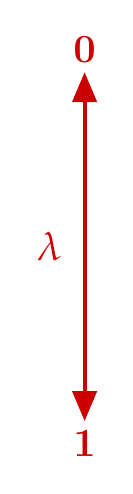
\begin{tikzpicture}
	\node[font = \Large, color = newred] at (0, 0) (uno){$\Unovet$};
	\node[font = \Large, color = newred] at (0, 5) (zero){$\Zerovet$};
	\draw[>=triangle 45, <->, line width=1.5pt, color = newred](uno) -- (zero) node [pos=.5, label=left:{\Large$\lambda$}, color = newred] {};
\end{tikzpicture}
\end{minipage}
\begin{minipage}{0.89\linewidth}
	\includegraphics[width = \linewidth]{img/shr_color.pdf}
\end{minipage}
\end{frame}

\begin{frame}[label = {app:shr2}]{\hyperlink{cap:reco}{Shrinking covariance matrix representation}}{
Hierarchical structure with $3$ time series and $m = 2$ with two different values of $\lambda\in\{0,1\}$, the shrinkage parameter}
\centering
\begin{minipage}{0.075\linewidth}\centering\vskip0.45cm
	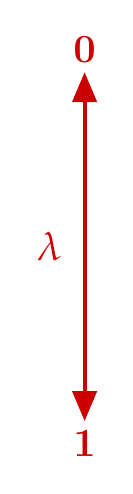
\begin{tikzpicture}
	\node[font = \Large, color = newred] at (0, 0) (uno){$\Unovet$};
	\node[font = \Large, color = newred] at (0, 5) (zero){$\Zerovet$};
	\draw[>=triangle 45, <->, line width=1.5pt, color = newred](uno) -- (zero) node [pos=.5, label=left:{\Large$\lambda$}, color = newred] {};
\end{tikzpicture}
\end{minipage}
\begin{minipage}{0.89\linewidth}
	\includegraphics[width = \linewidth]{img/shr_color2.pdf}
\end{minipage}
\end{frame}

\begin{frame}[label = {tab:es}]{\hyperlink{tab:crps}{ES ratio indices for the Australian Tourism Demand dataset}}{Red: worse than the benchmark (ctjb). Bold: the best for each column. Blue: the overall lowest value.}
\centering
\footnotesize
	\begin{tabular}[t]{l|>{}cccc>{}c|ccccc}
\toprule
\multicolumn{1}{c}{\textbf{}} & \multicolumn{10}{c}{\textbf{Generation of the base forecasts sample paths}} \\[-0.1cm]
\multicolumn{1}{c}{\makecell[c]{\bfseries Reconciliation\\\bfseries approach}} & \multicolumn{1}{c}{ctjb} & \multicolumn{4}{c}{\makecell[c]{Gaussian approach}} & \multicolumn{1}{c}{ctjb} & \multicolumn{4}{c}{\makecell[c]{Gaussian approach}} \\[-0.1cm]
\multicolumn{1}{c}{} &  & G & B & H & \multicolumn{1}{c}{HB} &  & G & B & H & HB\\
\midrule
\addlinespace[0.3em]
\multicolumn{1}{c}{} & \multicolumn{5}{c}{\textbf{$\forall k \in \{12,6,4,3,2,1\}$}} & \multicolumn{5}{c}{\textbf{$k = 1$}}\\
base & \textcolor{black}{1.000} & \textcolor{black}{0.956} & \textcolor{black}{0.955} & \textcolor{black}{0.958} & \textcolor{black}{0.951} & \textcolor{black}{1.000} & \textcolor{black}{0.952} & \textcolor{black}{0.950} & \textcolor{black}{0.952} & \textcolor{black}{0.950}\\
ct$(bu)$ & \textcolor{red}{2.427} & \textcolor{black}{0.983} & \textcolor{black}{0.983} & \textcolor{black}{0.983} & \textcolor{black}{0.983} & \textcolor{red}{1.759} & \textcolor{black}{0.982} & \textcolor{black}{0.982} & \textcolor{black}{0.982} & \textcolor{black}{0.982}\\
ct$(shr_{cs}, bu_{te})$ & \textcolor{red}{1.243} & \textcolor{black}{0.886} & \textcolor{black}{0.879} & \textcolor{black}{0.886} & \textcolor{black}{0.879} & \textcolor{red}{1.098} & \textcolor{black}{0.929} & \textcolor{black}{0.928} & \textcolor{black}{0.930} & \textcolor{black}{0.927}\\
ct$(wlsv_{te}, bu_{cs})$ & \textcolor{red}{1.499} & \textcolor{black}{0.977} & \textcolor{black}{0.977} & \textcolor{black}{0.971} & \textcolor{black}{0.972} & \textcolor{red}{1.241} & \textcolor{black}{0.975} & \textcolor{black}{0.975} & \textcolor{black}{0.973} & \textcolor{black}{0.974}\\
oct$(ols)$ & \textcolor{black}{0.955} & \textcolor{black}{0.893} & \textcolor{black}{0.891} & \textcolor{black}{0.893} & \textcolor{black}{0.888} & \textcolor{black}{0.975} & \textcolor{black}{0.937} & \textcolor{black}{0.936} & \textcolor{black}{0.936} & \textcolor{black}{0.935}\\
oct$(struc)$ & \textcolor{red}{1.085} & \textcolor{black}{0.917} & \textcolor{black}{0.915} & \textcolor{black}{0.916} & \textcolor{black}{0.912} & \textcolor{red}{1.027} & \textcolor{black}{0.943} & \textcolor{black}{0.942} & \textcolor{black}{0.943} & \textcolor{black}{0.942}\\
oct$(wlsv)$ & \textcolor{red}{1.132} & \textcolor{black}{0.933} & \textcolor{black}{0.929} & \textcolor{black}{0.931} & \textcolor{black}{0.927} & \textcolor{red}{1.050} & \textcolor{black}{0.951} & \textcolor{black}{0.949} & \textcolor{black}{0.950} & \textcolor{black}{0.949}\\
oct$(bdshr)$ & \textcolor{red}{1.047} & \textcolor{black}{0.904} & \textcolor{black}{0.897} & \textcolor{black}{0.897} & \textcolor{black}{0.891} & \textcolor{red}{1.009} & \textcolor{black}{0.936} & \textcolor{black}{0.933} & \textcolor{black}{0.934} & \textcolor{black}{0.931}\\
\bottomrule
\end{tabular}
\end{frame}


\begin{frame}[label = {app:pbu}]{\hyperlink{cap:reco}{Partly bottom up}}
\begin{minipage}{0.49\textwidth}
		\centering
		$\widetilde{\Xvet}$ with ct$(rec_{cs}, bu_{te})$\\
		\resizebox{\linewidth}{!}{
			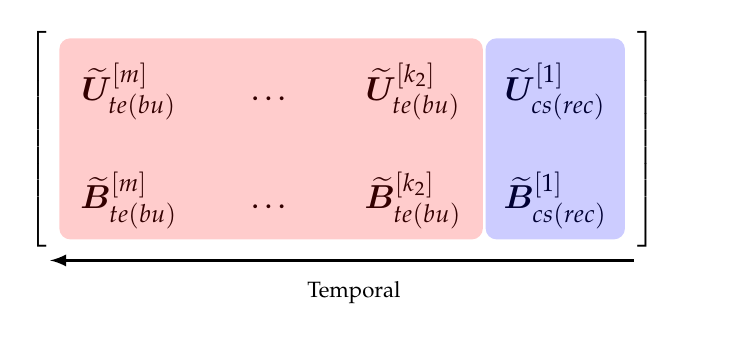
\begin{tikzpicture}[>=latex, line width=1pt,
				Matrix/.style={
				matrix of nodes,
				font=\large,
				align=center,
				text width = 1.5cm,
				text height = 0.65cm,
				column sep=2pt,
				row sep=7pt,
				nodes in empty cells,
				left delimiter={[},
						right delimiter={]},
						ampersand replacement=\&
						}]
				\matrix[Matrix] (Mt){ % Matrix contents
				$\widetilde{\Uvet}_{te(bu)}^{[m]}$ \& \dots \& $\widetilde{\Uvet}_{te(bu)}^{[k_2]}$ \& $\widetilde{\Uvet}_{cs(rec)}^{[1]}$ \\
				$\widetilde{\Bvet}^{[m]}_{te(bu)}$ \& \dots \& $\widetilde{\Bvet}^{[k_2]}_{te(bu)}$ \& $\widetilde{\Bvet}^{[1]}_{cs(rec)}$ \\
				};
				\draw[<-, opacity = 0] (Mt.north east)++(0.4,0) coordinate (temp) -- (temp |- Mt.south) node [midway,label={[label distance=0.1cm,rotate=-90, xshift = 1.5mm, font=\footnotesize]Cross-sectional}]{};
				\draw[<-] (Mt.south west)++(0,-0.15) coordinate (temp) -- (temp -| Mt.east) node [midway,label={[label distance=0cm,xshift = 1.5mm, font=\footnotesize]below:Temporal}]{};
				\node[opacity=0.2,
					rounded corners,
					inner sep=0pt, fill = blue, fit=(Mt-1-4)(Mt-2-4)](Bt){};
				\node[opacity=0.2,
					rounded corners,
					inner sep=0pt, fill = red, fit=(Mt-1-1)(Mt-2-3)](At){};
			\end{tikzpicture}}
\end{minipage}
\begin{minipage}{0.49\textwidth}
		\centering
		$\widetilde{\Xvet}$ with ct$(rec_{te}, bu_{cs})$\\
		\resizebox{\linewidth}{!}{
			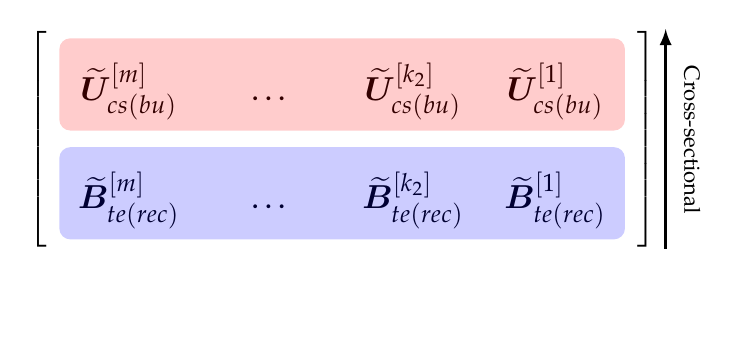
\begin{tikzpicture}[>=latex, line width=1pt,
				Matrix/.style={
				matrix of nodes,
				font=\large,
				align=center,
				text width = 1.5cm,
				text height = 0.65cm,
				column sep=2pt,
				row sep=7pt,
				nodes in empty cells,
				left delimiter={[},
						right delimiter={]},
						ampersand replacement=\&
						}]
				\matrix[Matrix] (Mcs){ % Matrix contents
				$\widetilde{\Uvet}_{cs(bu)}^{[m]}$ \& \dots \& $\widetilde{\Uvet}_{cs(bu)}^{[k_2]}$ \& $\widetilde{\Uvet}_{cs(bu)}^{[1]}$ \\
				$\widetilde{\Bvet}^{[m]}_{te(rec)}$ \& \dots \& $\widetilde{\Bvet}^{[k_2]}_{te(rec)}$ \& $\widetilde{\Bvet}^{[1]}_{te(rec)}$ \\
				};
				\draw[<-] (Mcs.north east)++(0.4,0) coordinate (temp) -- (temp |- Mcs.south) node [midway,label={[label distance=0.1cm,rotate=-90, xshift = 1.5mm, font=\footnotesize]Cross-sectional}]{};
				\draw[<-, opacity = 0] (Mcs.south west)++(0,-0.15) coordinate (temp) -- (temp -| Mcs.east) node [midway,label={[label distance=0cm,xshift = 1.5mm, font=\footnotesize]below:Temporal}]{};
				\node[opacity=0.2,
					rounded corners,
					inner sep=0pt, fill = blue, fit=(Mcs-2-1)(Mcs-2-4)](Bcs){};
				\node[opacity=0.2,
					rounded corners,
					inner sep=0pt, fill = red, fit=(Mcs-1-1)(Mcs-1-4)](Acs){};
			\end{tikzpicture}}
\end{minipage}
\begin{itemize}[itemsep = 0.25cm]
	\item The \colorbox{mybluehl}{blue} background indicates generating reconciled forecasts along one dimension, while the \colorbox{pink}{pink} background indicates the forecasts obtained using bottom-up along the other
	\item[\textbf{L}] {\color{blue}Cross-sectionally} reconciled forecasts for $k=1$ ($\widetilde{\Uvet}^{[1]}$ and $\widetilde{\Bvet}^{[1]}$) followed by {\color{newpink}temporal} bottom-up
	\item[\textbf{R}] {\color{blue}Temporally} reconciled forecasts of the cross-sectional bottom time series $(\widetilde{\Bvet}^{[k]}, \, k\in \mathcal{K})$ followed by {\color{newpink}cross-sectional} bottom-up
\end{itemize}
\end{frame}

\begin{frame}[label = {app:cov}]{\hyperlink{cap:reco}{Cross-temporal covariance approximations}}{\cite{difonzo2023}\hspace{0.675\linewidth}\hyperlink{cap:opt}{\faArrowRight}}
\begin{itemize}[leftmargin=!, labelwidth=\widthof{ oct$(bdsam)$ -}, align=right]
	\item[oct$(ols)$ -] identity: $\Omegavet_{ct} = \Ivet_{n(k^*+m)}$
	\item[oct$(struc)$ -] structural: $\Omegavet_{ct} = \mathrm{diag}(\Fvet \mathbf{1}_{mn_b})$
	\item[oct$(wlsv)$ -] series variance scaling: $\Omegavet_{ct} = \widehat{\Omegavet}_{ct,wlsv}$, a straightforward extension of the series variance scaling matrix presented by \cite{athanasopoulos2017}
	\item[oct$(bdshr)$ -] block-diagonal shrunk cross-covariance scaling: $\Omegavet_{ct} = \Pvet\widehat{\Wvet}^{BD}_{ct,shr}\Pvet'$, with $\widehat{\Wvet}^{BD}_{ct,shr}$ a block diagonal matrix where each $k-$block ($k = m,k_{p-1},\dots, 1$) is $\Ivet_{M_k} \otimes \widehat{\Wvet}^{[k]}_{shr}$, $\widehat{\Wvet}^{[k]}_{shr}$ is the shrunk estimate of the cross-sectional covariance matrix proposed by \cite{wickramasuriya2019}, and $\Pvet$ is the commutation matrix such that $\Pvet \text{vec}(\Yvet_{\tau}) = \text{vec}(\Yvet_{\tau}')$
	\item[oct$(shr)$ -] MinT-shr:   $\Omegavet_{ct} = \hat{\lambda}\widehat{\Omegavet}_{ct,D} + (1-\hat{\lambda})\widehat{\Omegavet}_{ct}$,
	where $\hat{\lambda}$ is an estimated shrinkage coefficient (\citealp{ledoit2004a}), $\widehat{\Omegavet}_{ct,D} = \Ivet_{n(k^\ast + m)} \odot \widehat{\Omegavet}_{ct}$ with $\odot$ denoting the Hadamard product, and $\widehat{\Omegavet}_{ct}$ is the covariance matrix of the cross-temporal one-step ahead in-sample forecast errors
\end{itemize}
\end{frame}

\begin{frame}[label = {tab:mcb}]{\hyperlink{tab:crps}{Gaussian vs bootstrap MCB Nemenyi test}}{Comparison between base and the best reconciled forecasts using gaussian $\Box$ and bootstrap $\Large\circ$ approaches}
	\includegraphics[width = \linewidth]{img/slide_mcb1.pdf}

\begin{tikzpicture}[overlay,remember picture]
\draw [black, line width=5mm, opacity = 0.15] (0.9,5.05) -- (3.2,5.05);
\draw [black, line width=5mm, opacity = 0.15] (0.9,5.65) -- (3.2,5.65);
\draw [newred, line width=5mm, opacity = 0.15] (0.2,4.45) -- (3.2,4.45);
\draw [newred, line width=5mm, opacity = 0.15] (0.2,3.85) -- (3.2,3.85);
\draw [newred, line width=5mm, opacity = 0.15] (0.2,3.25) -- (3.2,3.25);
\draw [newblue, line width=5mm, opacity = 0.15] (0.6,2.65) -- (3.2,2.65);
\draw [newblue, line width=5mm, opacity = 0.15] (0.2,2.05) -- (3.2,2.05);
\draw [newblue, line width=5mm, opacity = 0.15] (0.1,1.45) -- (3.2,1.45);
\end{tikzpicture}
\end{frame}

\begin{frame}[label = {app:multi}]{\hyperlink{cap:samples}{From one- to multi-step residuals}}
\begin{minipage}{0.32\linewidth}
	\includegraphics[width = \linewidth]{img/multi_one_slide.pdf}
\end{minipage}\hfill
\begin{minipage}{0.6\linewidth}
	\begin{itemize}[leftmargin = 0cm, itemsep = 0.2cm]
	\item Model residuals may be used to estimate the covariance matrix for the base forecasts $\Omegavet$ or for the reconciled formula $\Omegavet_{ct}$
	\item In time series analysis, it is common to use residuals corresponding to {\color{newred}one-step ahead} forecasts
	\item Due to the temporal dimension, residuals corresponding to {\color{avocado}different forecast horizons} are required
	\item \textbf{\color{newblue}Multi-step residuals} 
	$$e_{i,h,j}^{[k]} = x_{i,j+h}^{[k]} - \widehat{x}_{i,j+h|j}^{[k]},$$
	where $\widehat{x}_{i,j+h|t}^{[k]}$ is the $h$-step fitted value.
	\item In general, these residuals will be \textbf{\color{avocado}autocorrelated} except \\when $h=1$ (one-step residuals)
\end{itemize}
\end{minipage}\hspace{0.25cm}
\end{frame}


\begin{frame}[label = {app:sntz}]{\hyperlink{cap:fexp}{Dealing with negativity issues: set-negative-to-zero}}
	\begin{itemize}[itemsep = 0.25cm]
		\item {\color{newred}One issue} in working with time series data is the presence of {\color{newred}negative values}, which can cause difficulties for certain types of models or analyses
		\item Cross-sectional {\color{avocado}non negative reconciliation}: \cite{wickramasuriya2020}
		\item {\color{avocado}Non negative cross-temporal reconciliation} proposed by \cite{difonzo2022b, difonzo2023a}
		\begin{itemize}[label = $\bullet$, itemsep = 0.1cm]
		\item State-of-the-art numerical {\color{avocado}optimization} procedure (osqp, \citealp{stellato2020})
		\item Simple {\color{avocado}heuristic} strategy: set-negative-to-zero (sntz)
		\begin{enumerate}
			\item Negative high-frequency bottom ts reconciled forecasts are set to zero $\rightarrow \widetilde{\bvet}_0^{[1]}$
			\item Apply cross-temporal bottom-up to obtain fully coherent non negative forecasts
		\end{enumerate}
		\end{itemize}
		$$
{\color{newred}\underset{\parbox[t]{2.5cm}{\small\centering\vskip0.05mm Incoherent}}{\widehat{\xvet}}} \rightarrow {\color{newblue}\underset{\parbox[t]{2.5cm}{\small\centering\vskip0.05mm Coherent}}{\widetilde{\xvet}}} \rightarrow {\color{avocado}\underset{\parbox[t]{4cm}{\small\centering\vskip0.05mm Not negative and coherent}}{\widetilde{\xvet}_0 = \Fvet \widetilde{\bvet}_0^{[1]}}}
$$
		\item[\faPlus] Sntz requires much {\color{avocado}less time and computational effort} than optimization
		\item[\faPlus] In the empirical application, both sntz and osqp produce {\color{avocado}similar quality forecasts} 
	\end{itemize}
\end{frame}

\end{document}